\documentclass[11pt,a4paper]{report}
\usepackage{graphicx,epsfig}
\usepackage{amsfonts}
\usepackage{amsthm, amsmath}
\usepackage{xcolor}
\usepackage{textcomp}
\usepackage{listings}
\usepackage[authoryear,round]{natbib}
\usepackage[hidelinks]{hyperref}
\usepackage{todonotes}
\usepackage{mathtools}
\usepackage[ruled]{algorithm2e}
\usepackage{graphicx}
\usepackage{svg}
\usepackage{tabularx}
\usepackage{pdfpages}
\usepackage[nameinlink]{cleveref}

\usepackage{geometry}
\geometry{margin=2cm}

\newcommand*\diff{\mathop{}\!\mathrm{d}}
\DeclareMathOperator{\trace}{trace}
\DeclareMathOperator{\diag}{diag}
\DeclareMathOperator*{\argmax}{arg\,max}
\DeclareMathOperator*{\argmin}{arg\,min}

\newcolumntype{Y}{>{\centering\arraybackslash}X}

\graphicspath{ {./figures/} }

\parindent=25pt
\parskip 0.10in

\date{}
\begin{document}

\newgeometry{top=8cm}

\thispagestyle{empty}
\begin{center}
{\huge
Gradient-Free Optimal Postprocessing \\
of MCMC Output

\bigskip
\bigskip

by
\bigskip
\bigskip

Artem Glebov
}
\end{center}
\vfill

\begin{center}
{\large
Department of Mathematics\\
King's College London\\
The Strand, London WC2R 2LS\\
United Kingdom\\
\medskip

}
\end{center}
\bigskip


\newpage
\setcounter{page}{1}
\restoregeometry

\chapter*{Abstract}

The dissertation reports the results of implementing the gradient-free kernel Stein discrepancy of \cite{fisherGradientFreeKernelStein2024} within the Stein thinning algorithm of \cite{riabizOptimalThinningMCMC2022}. We evaluate the performance of the proposed algorithm on a Gaussian mixture target distribution and in a Bayesian inverse problem for the Lotka-Volterra model. The results confirm the feasibility of the proposed algorithm and highlight the primary challenge in its practical application: the requirement for an auxiliary distribution to be provided by the user.


\tableofcontents


\chapter*{Introduction}

The Stein thinning algorithm was recently proposed by \cite{riabizOptimalThinningMCMC2022}, motivated by the problem of selecting a subsample from Markov Chain Monte Carlo (MCMC) output for further expensive processing. The algorithm relies on the kernel Stein discrepancy (KSD), whose calculation involves the gradients of the log-density of the target distribution. The requirement to provide the gradients imposes a significant computational cost on the practitioner attempting to use it for non-trivial distributions, such as posteriors in Bayesian inverse problems. \cite{fisherGradientFreeKernelStein2024} developed a way around this challenge by formulating a gradient-free version of KSD, which the authors applied in the context of importance sampling and variational inference.

We adopt the proposal of \cite{fisherGradientFreeKernelStein2024} to implement a gradient-free version of the original Stein thinning algorithm, and evaluate the newly developed algorithm on simple but illustrative cases of the Gaussian mixture and Bayesian inference for the parameters of the Lotka-Volterra model, demonstrating the feasibility of the algorithm, and highlighting practical challenges for its application.

The report is organised as follows. \Cref{ch:background} reviews MCMC methods and discusses the challenges of applying MCMC to practical problems. It proceeds to explain how the Stein thinning algorithm of \cite{riabizOptimalThinningMCMC2022} offers a solution for retrospective bias removal and compression of samples. The gradient-free KSD of \cite{fisherGradientFreeKernelStein2024} is then introduced. \Cref{ch:methodology} describes our proposed approach, supported by numerical experiments. Finally, \Cref{ch:conclusions} summarises the finding of the experiments and suggests ideas for further research. Additional derivations and figures are included in the Appendices.

The Python code reproducing the experiments in this report can be found at:
\begin{center}
\vspace{-10pt}
\url{https://github.com/aglebov/gradient-free-mcmc-postprocessing}.
\vspace{-10pt}
\end{center}
The implementation of the gradient-free kernel Stein thinning was contributed by the author directly to the \texttt{stein-thinning} Python library:
\begin{center}
\vspace{-10pt}
\url{https://github.com/wilson-ye-chen/stein_thinning}.
\end{center}

\chapter*{Notation}

For a matrix $A$, we use use $A^T$ to denote the transpose of $A$. The matrix $A^{1/2}$ is called the square root of $A$ if it satisfies $A^{1/2} A^{1/2} = A$. $A^{-1}$ is the inverse of $A$, if it exists. $I$ stands for the identity matrix of an appropriate dimension.

We use $\langle x, y \rangle$ to denote the scalar product of $x$ and $y$, and $\| x \|$ to denote the norm of $x$.

For a function $f: \mathbb{R}^d \to \mathbb{R}$, $\nabla f(x)$ denotes the gradient of $f(x)$, given by the vector
\begin{equation*}
\nabla f(x) \coloneq \left( \frac{\partial f(x)}{\partial x_1}, \dots, \frac{\partial f(x)}{\partial x_d} \right)^T,
\end{equation*}
where $x_i$ are the components of $x$ for $i \in \{1, \dots, d\}$.
For a function of two arguments $f(x, y): \mathbb{R}^d \times \mathbb{R}^d \to \mathbb{R}$, we define gradients w.r.t.\ each argument:
\begin{equation*}
\begin{aligned}
\nabla_x f(x, y) &\coloneq \left(\frac{\partial f(x, y)}{\partial x_1}, \dots, \frac{\partial f(x, y)}{\partial x_d}\right)^T, \\
\nabla_y f(x, y) &\coloneq \left(\frac{\partial f(x, y)}{\partial y_1}, \dots, \frac{\partial f(x, y)}{\partial y_d}\right)^T, \\
\end{aligned}
\end{equation*}
where $x_i$ and $y_i$ are the components of $x$ and $y$, respectively, for $i \in \{1, \dots, d\}$. The operator $\nabla_x \cdot \nabla_y$ is then defined as
\begin{equation*}
(\nabla_x \cdot \nabla_y) f(x,y) \coloneq \sum_{i=1}^d \frac{\partial^2}{\partial x_i\, \partial y_i} f(x, y).
\end{equation*}

The probability of an event $A$ is denoted by $\mathbb{P}(A)$. For a sequence of probability measures $P_m$ and a probability measure $P$ on a measurable space $\mathcal{X}$, $P_m \xrightarrow[]{d} P$ as $m \to \infty$ denotes weak convergence:
\begin{equation*}
\int_{\mathcal{X}} f \diff P_m \to \int_{\mathcal{X}} f \diff P \quad \text{as } m \to \infty \quad \text{for all bounded, continuous functions } f.
\end{equation*}

We use the common abbreviation ``i.i.d.'' for ``independent and identically distributed'' in relation to random variables.


\chapter{Background}
\label{ch:background}

\section{Markov chain Monte Carlo (MCMC)}

Markov chain Monte Carlo (MCMC) are a popular class of algorithms for sampling from complex probability distributions.

The need to sample from a probability distribution arises in exploratory analysis as well as when analytical expressions are unavailable for quantities of interest, such as the modes or quantiles of the distribution, or for expectations with respect to the distribution, so a Monte Carlo simulation is used to obtain approximations instead. Such cases are frequent in Bayesian analysis, where the posterior density often has a complex structure with an analytically intractable normalising constant.

In the simplest cases where the inverse cumulative density function of a distribution is available, sampling can be done using the straightforward inverse method. Bespoke sampling methods, such as the Box-Muller transform for the normal distribution, can occasionally be developed by exploiting the properties of specific distributions. When a bespoke strategy is unavailable, the accept-reject algorithm and importance sampling offer an alternative, provided one can find an auxiliary distribution that approximates the target sufficiently well and that is easy to sample from. See Chapters 2 and 3 in \cite{robertMonteCarloStatistical2004} for an overview of these methods. In many cases, however, the complexity of the target distribution and the dimensionality of the parameter space render these methods infeasible or inefficient. The class of MCMC algorithms has arisen to address the challenge.

Given a target distribution $P$ defined on a state space $\mathcal{X}$, an MCMC algorithm proceeds by constructing a chain of random variables $(X_i)_{i=0}^\infty$  which satisfy the Markov property:
\begin{equation*}
\mathbb{P}(X_{i+1}\in A | X_0, \dots, X_i) = \mathbb{P}(X_{i+1}\in A | X_i) \quad\text{for any measurable } A \in \mathcal{X}.
\end{equation*}
Viewed as a function, the right-hand side above is called the Markov transition kernel and is denoted 
\begin{equation}
R(A | x) \coloneq \mathbb{P}(X_{i+1}\in A | X_i = x).
\end{equation}
If the transition kernel does not depend on the index $i$, the marginal distribution of $X_{i+1}$ is given by the recursive relationship
\begin{equation*}
P_{i+1}(A) \coloneq \mathbb{P}(X_{i+1} \in A) = \int_{\mathcal{X}} R(A|x) P_i(\diff x) \quad\text{for } i = 0, 1, \dots
\end{equation*}
The initial value $X_0$ is assumed to come from some known distribution $P_0$.
The transition kernel $R$ is selected so that it is easy to sample from and to ensure asymptotic convergence to the target distribution $P$:
\begin{equation*}
P_i \xrightarrow[]{d} P \quad\text{as}\quad i \to \infty.
\end{equation*}
A sample of size $n$ is a realisation $(x_i)_{i=0}^n$ of the first $n$ variables in the chain, which is constructed sequentially.

Two classical variations of this technique are the Metropolis-Hastings and Gibbs algorithms.

\paragraph{Metropolis-Hastings algorithm.} The algorithm due to \cite{metropolisEquationStateCalculations1953} and \cite{hastingsMonteCarloSampling1970} uses an auxiliary distribution $q$ to sample a proposed value\footnote{Note that here we discuss the algorithm which operates on realisations of random variables, so we use lowercase letters to denote the realised values.}
$$x' \sim q(x' | x_i),$$
which is then accepted with probability
$$\alpha(x_i, x') = 1 \wedge \frac{p(x')}{p(x_i)} \frac{q(x_i|x')}{q(x'|x_i)},$$
where $p$ is the density of the target distribution $P$.
If $x'$ is accepted, the algorithm sets $x_{i+1} = x'$. If $x'$ is rejected, the value remains unchanged: $x_{i+1} = x_i$.

The common choice for $q$ is symmetric satisfying $q(x'|x_i) = q(x_i|x')$, so that the ratio of these two quantities disappears from the expression for the acceptance probability:
$$\alpha(x_i, x') = 1 \wedge \frac{p(x')}{p(x_i)}.$$
In the special case where $q(x'|x_i) = q(x' - x_i)$ we obtain a random walk proposal:
$$x' = x_i + z.$$
The step $z$ is sampled from the proposal distribution of the algorithm, such as the multivariate normal distribution. The operation of the algorithm then resembles a random walk across the domain of the target distribution where steps towards areas of higher probability are more likely to be accepted. The scale of the step distribution determines the average size of the jump that the algorithm can make at each iteration and thus the speed of traversal of the target domain. Choosing a good value for the step size is one of the practical hurdles one must address when using this algorithm, as we discuss in \Cref{sec:background:challenges}. An alternative to symmetric proposals is an independence proposal satisfying $q(x'|x_n) = q(x')$.

\paragraph{Gibbs algorithm.} Suppose $x$ is a $d$-dimensional vector with components $(x^{(1)}, \dots, x^{(d)})$ and that the conditional distributions $f_k(x^{(k)} | x^{(1)}, \dots, x^{(k-1)}, x^{(k+1)}, \dots, x^{(d)})$ for $k \in \{1, \dots, d\}$ are easy to sample from. The draw $x_{i+1}$ can then be constructed by sampling each component in turn while keeping the other components fixed, that is
\begin{equation*}
\begin{aligned}
x_{i+1}^{(1)} &\sim f_1(x^{(1)} | x_{i}^{(1)}, \dots, x_{i}^{(d)}), \\
x_{i+1}^{(2)} &\sim f_2(x^{(2)} | x_{i+1}^{(1)}, x_{i}^{(3)} \dots, x_{i}^{(d)}), \\
\vdots \\
x_{i+1}^{(k)} &\sim f_k(x^{(k)} | x_{i+1}^{(1)}, \dots, x_{i+1}^{(k-1)}, x_{i}^{(k+1)} \dots, x_{i}^{(d)}), \\
\vdots \\
x_{i+1}^{(d)} &\sim f_d(x^{(d)} | x_{i+1}^{(1)}, \dots, x_{i+1}^{(d-1)}).
\end{aligned}
\end{equation*}
Unlike the Metropolis-Hastings algorithm, the Gibbs sampler does not require a proposal distribution $q$. It might, however, be slower to converge and is prone to getting trapped in the vicinity of the nearest mode (see Section 10.3.1 in \cite{robertMonteCarloStatistical2004}).

While the Metropolis-Hastings algorithm accesses the target distribution only via evaluation of $p(x)$, more recent MCMC techniques take advantage of the additional information available from the gradient of $p(x)$: the Metropolis-adjusted Langevin Algorithm (MALA) adds a bias to the proposal distribution in the direction of $\nabla \log p(x)$ (Section 2.1.4 in \cite{fearnheadScalableMonteCarlo2024}), and the Hamiltonian Monte Carlo (HMC) algorithm treats $-\log p(x)$ as the potential energy field and simulates the movement of a particle whose momentum is determined by $\nabla \log p(x)$ (Section 2.2 in \cite{fearnheadScalableMonteCarlo2024}).

Development of general-purpose and specialised MCMC algorithms remains an active area of research, with particular focus on scalability (\cite{fearnheadScalableMonteCarlo2024}).

\section{Challenges of running MCMC}
\label{sec:background:challenges}

While the asymptotic convergence of MCMC samples to the target distribution is guaranteed, no general guarantee is available for finite samples, resulting in several interrelated challenges that a practitioner faces when applying this class of algorithms:
\begin{enumerate}
\item The choice of a starting point for a chain affects the speed of convergence to the target distribution.
\item For a multimodal distribution, the algorithm might struggle to move between the modes within a feasible time. This problem becomes especially acute in high dimensions.
\item The scale of the proposal distribution must be calibrated to ensure that the algorithm is able to explore the domain of the target distribution efficiently.
\item Assessing how close an MCMC chain is to convergence is difficult, since the knowledge about the target distribution often comes from the chain itself.
\item In order to eliminate the impact of the starting point, it can be useful to discard the initial iterations of an MCMC chain, which are considered as ``burn-in''. Selecting the optimal length of the burn-in period is contingent on being able to detect convergence.
\item The sequential procedure of constructing a chain introduces autocorrelation between the samples, which leads to increased variance of resulting estimators.
\item The large number of samples resulting from an MCMC algorithm might need to be summarised for subsequent analysis, particularly when the cost of using all available samples is too high. Such situations arise when samples obtained from MCMC are used as starting points for further expensive simulations.
\end{enumerate}

The first three challenges require decisions to be made upfront before running the algorithm or adaptively during its run. In order to address the impact of the starting point, running multiple chains with starting points sampled from an overdispersed distribution is recommended~(\cite{gelmanInferenceIterativeSimulation1992}). This approach has the added benefit of increasing the chance of discovering the modes of the target distribution, although it does not provide a guarantee in this respect. 

The scaling of the step distribution in the random-walk Metropolis-Hastings algorithm is commonly tuned to target the acceptance rate of roughly 0.234 for proposed samples (\cite{gelmanEfficientMetropolisJumping1996,gelmanWeakConvergenceOptimal1997,robertsOptimalScalingVarious2001}), which balances the speed of traversal and the computational effort generating samples that end up rejected.

Comparing the summary statistics of several chains (\cite{gelmanInferenceIterativeSimulation1992,brooksGeneralMethodsMonitoring1998,vehtariRankNormalizationFoldingLocalization2021}) offers a way to detect a lack of convergence at the cost of additional computation. Alternatively, the comparison can be applied to batches of samples from a single chain, as proposed by \cite{vatsRevisitingGelmanRubin2021}. Convergence detection can be used to terminate the algorithm once a chosen criterion is satisfied. It should be noted that convergence criteria establish a necessary but not sufficient condition for convergence, so the outcomes need to be interpreted accordingly.

The last three challenges are typically addressed by post-processing a sample from a completed MCMC run. A recent proposal by~\cite{riabizOptimalThinningMCMC2022} addresses these challenges by selecting a fixed-size subset of samples from an MCMC run such that the empirical distribution given by the subset best approximates the target distribution. In the following section, we consider their approach in greater detail.

\section{Stein thinning}
\label{sec:stein-thinning}

Given MCMC output $(x_i)_{i=1}^n$ of length $n$, the empirical approximation of the target distribution is
\begin{equation}
\frac{1}{n} \sum_{i=1}^n \delta(x_i),
\label{eq:discrete-distribution}
\end{equation}
where $\delta(x)$ is the Dirac delta function.
\cite{riabizOptimalThinningMCMC2022} set out to identify $m \ll n$ indices $\pi(j) \in \{1,\dots, n\}$ with $j\in\{1, \dots, m\}$, such that the approximation provided by the subset of samples
\begin{equation}
\frac{1}{m} \sum_{j=1}^m \delta(x_{\pi(j)})
\label{eq:thinned-sample}
\end{equation}
is closest to the target distribution. The criterion of proximity is based on the kernel Stein discrepancy, itself a special case of the integral probability metric.

The integral probability metric (\cite{mullerIntegralProbabilityMetrics1997}) between two distributions $P$ and $P'$ is defined as
\begin{equation}
\mathcal{D}_{\mathcal{F}}(P, P') \coloneq \sup_{f \in \mathcal{F}}\left|\int_\mathcal{X} f \diff P - \int_\mathcal{X} f \diff P' \right|,
\label{eq:ipm}
\end{equation}
where $\mathcal{X}$ is a measurable space on which both $P$ and $P'$ are defined and $\mathcal{F}$ is a set of test functions. The set $\mathcal{F}$ needs to be rich enough to detect differences between $P$ and $P'$, ensuring that
\begin{equation*}
\mathcal{D}_{\mathcal{F}}(P, P') = 0 \quad \text{iff} \quad P = P',
\end{equation*}
in which case the metric is said to be measure determining.
%Depending on the choice of $\mathcal{F}$, the definition~(\ref{eq:ipm}) gives rise to different classes of probability metrics, including the well-known Kolmogorov distance, Wasserstein distance and total variation distance.
Furthermore, it is desirable for the metric to provide convergence control, so that
\begin{equation*}
\mathcal{D}_{\mathcal{F}}(P, P'_m) \to 0 \quad \text{implies} \quad P'_m \xrightarrow[]{d} P
\end{equation*}
as $m \to \infty$, for any sequence of distributions $P'_m$.

If $P$ is taken to be the target distribution of an MCMC algorithm, evaluating~(\ref{eq:ipm}) poses two practical challenges: the integral $\int_\mathcal{X} f \diff P$ is often analytically intractable, and the supremum requires a non-trivial optimisation procedure to find.

The need to integrate with respect to $P$ can be eliminated if we find a set of function $\mathcal{F}$, such that $\int_\mathcal{X} f \diff P = 0$ for all $f \in \mathcal{F}$. The expression~(\ref{eq:ipm}) then simplifies to
\begin{equation}
\mathcal{D}_{\mathcal{F}}(P, P') = \sup_{f \in \mathcal{F}}\left|\int_\mathcal{X} f \diff P' \right|.
\label{eq:stein-discrepancy-sup}
\end{equation}

\cite{gorhamMeasuringSampleQuality2015} propose choosing such a set $\mathcal{F}$ based on the observation that the infinitesimal generator
$$(\mathcal{L}u)(x) \coloneq \lim_{t \to 0} \frac{\mathbb{E}[u(Z_t) | Z_0 = x] - u(x)}{t} \quad \text{for } u:\mathbb{R}^d \to \mathbb{R}$$
of a Markov process $(Z_t)_{t \geq 0}$ with stationary distribution $P$ satisfies 
\begin{equation}
\mathbb{E}[(\mathcal{L} u)(Z)] = 0
\label{eq:infinitesimal:property}
\end{equation}
under mild conditions on $\mathcal{L}$ and $u$. In the specific case of an overdamped Langevin diffusion
$$\diff Z_t = \frac{1}{2} \nabla \log p(Z_t) \diff t + \diff W_t,$$
where $p$ is the density of $P$ and $W_t$ is the standard Brownian motion, the infinitesimal generator becomes
$$(\mathcal{L}_P u)(x) = \frac{1}{2} \langle \nabla u(x), \nabla \log p(x)\rangle + \frac{1}{2}\langle \nabla, \nabla u(x) \rangle.$$
Denoting $g  = \frac{1}{2}\nabla u$, \cite{gorhamMeasuringSampleQuality2015} obtain the Stein operator
\begin{equation}
\mathcal{A}_P g \coloneq \langle g, \nabla \log p \rangle + \langle \nabla, g \rangle = \langle p^{-1}\nabla, p g \rangle,
\label{eq:stein-operator}
\end{equation}
and rewrite~(\ref{eq:stein-discrepancy-sup}) via~(\ref{eq:infinitesimal:property}) as
\begin{equation}
\mathcal{D}_{P, \mathcal{G}}(P') = \sup_{g \in \mathcal{G}}\left|\int_\mathcal{X} \mathcal{A}_P g \diff P' \right|
\label{eq:stein-discrepancy-g}
\end{equation}
for a suitably chosen set $\mathcal{G}$. The expression~(\ref{eq:stein-discrepancy-g}) defines the \textit{Stein discrepancy}. Since $p$ only appears in~(\ref{eq:stein-operator}) through $\nabla \log p$, the normalising constant of $p$ is not required to evaluate $\mathcal{D}_{P, \mathcal{G}}(P')$: for any constant $c > 0$ we have $\nabla \log (c p(x)) = \nabla \log p(x)$.

To remove the optimisation step in the calculation of~(\ref{eq:stein-discrepancy-g}), \cite{gorhamMeasuringSampleQuality2017} turn to reproducing kernel Hilbert spaces (RKHS). Recall that a vector space $V$ equipped with an inner product operation $\langle \cdot, \cdot \rangle$ and its induced norm $\|\cdot\|$ satisfying $\|v\|^2 = \langle v, v \rangle$ for all vectors $v$ in $V$, is called a Hilbert space if it is complete in the sense that
\begin{equation*}
\sum_{i=1}^\infty \|v_i\| < \infty \quad \text{implies} \quad \sum_{i=1}^\infty v_i \in V
\end{equation*}
for any sequence $v_i \in V$. A Hilbert space $\mathcal{H}$ of real-valued functions defined on a set $\mathcal{X}$ is called a \textit{reproducing kernel Hilbert space} if there exists a function $k: \mathcal{X} \times \mathcal{X} \to \mathbb{R}$ such that: (1) for every $x \in \mathcal{X}$, the function $k(x, \cdot)$ belongs to $\mathcal{H}$, (2) $k$ satisfies the reproducing property $\langle f(\cdot), k(\cdot, x)\rangle = f(x)$ for any $f \in \mathcal{H}$ and $x \in \mathcal{X}$. See Section 6.1 in \cite{rasmussenGaussianProcessesMachine2006} and Section 1.5 in \cite{fearnheadScalableMonteCarlo2024} for further discussion. We denote by $\mathcal{H}(k)$ the RKHS associated with kernel~$k$.

Taking the set
\begin{equation}
\mathcal{G} \coloneq \left\{ \mathrm{g} : \mathbb{R}^d \to \mathbb{R}^d \left| \sum_{i=1}^d \|g_i\|^2_{\mathcal{H}(k)} \leq 1 \right.\right\}
\label{eq:unit-ball}
\end{equation}
which defines a unit-ball in a Cartesian product of $d$ copies $\mathcal{H}(k)$, Proposition~2 in \cite{gorhamMeasuringSampleQuality2017} establishes that
\begin{equation}
\mathcal{D}_{P}^2(P') \coloneq \mathcal{D}_{P, \mathcal{G}}(P') = \iint_\mathcal{X} k_P(x, y) \diff p'(x) \diff p'(y),
\label{eq:stein-discrepancy-sqrt-expectation}
\end{equation}
where $p'$ is the density of $P'$, and $k_P(x, y)$ is given by
\begin{equation}
\begin{aligned}
k_P(x, y) \coloneq 
&(\nabla_x\cdot\nabla_y) k(x,y) \\
&+ \langle \nabla_x k(x, y), \nabla_y \log p(y) \rangle + \langle \nabla_y k(x, y), \nabla_x \log p(x) \rangle \\
&+ k(x, y) \langle \nabla_x \log p(x), \nabla_y \log p(y) \rangle.
\label{eq:deriv:stein-kernel}
\end{aligned}
\end{equation}
Expression~(\ref{eq:stein-discrepancy-sqrt-expectation}) thus defines the \textit{kernel Stein discrepancy} (KSD).
If $P'$ is a discrete distribution, as in~(\ref{eq:discrete-distribution}), the squared KSD becomes
\begin{equation}
\mathcal{D}_{P}^2\left(\frac{1}{n} \sum_{i=1}^n \delta(x_i)\right) = \frac{1}{n^2} \sum_{i,j=1}^n k_P(x_i, x_j),
\label{eq:ksd:discrete}
\end{equation}
i.e.\ the average of the elements in the Gram matrix of $k_P(x_i, x_j)$, which is straightforward to compute.

When $k(x, y)$ is chosen to be the inverse multiquadric kernel (IMQ)
\begin{equation}
k(x, y) = \left(c^2 + \|\Gamma^{-1/2}(x-y)\|\right)^\beta
\label{eq:imq}
\end{equation}
with $\beta \in (-1, 0)$ and $\Gamma = I$, \cite{gorhamMeasuringSampleQuality2017} demonstrate that $\mathcal{D}_{P}(P')$ provides convergence control (Theorem 8). Theorem 4 in \cite{chenSteinPointMarkov2019} justifies the introduction of $\Gamma$ in IMQ. The expression for $k_P(x, y)$ when $k(x, y)$ is taken to be the inverse multiquadric kernel is derived in Appendix~\ref{appendix:derivations:imq-stein}.

The hyperparameters $c$, $\Gamma$ and $\beta$ in~(\ref{eq:imq}) must be provided by the user. The constant $c$ in~(\ref{eq:imq}) can be set to 1 without loss of generality, and the positive-definite preconditioner matrix $\Gamma$ can be chosen to exploit the geometry of the parameter space. \cite{riabizOptimalThinningMCMC2022} suggest several choices for $\Gamma$, for instance the identity matrix scaled by the median Euclidean distance between points in the sample, which performed well in their experiments. \cite{gorhamMeasuringSampleQuality2017} and \cite{riabizOptimalThinningMCMC2022} both settle on the value $\beta = -\frac12$ based on empirical evaluation.

Other choices of kernels are possible and offer convergence control, as demonstrated by \cite{chenSteinPoints2018}, however IMQ performed on par or better than the alternatives considered by the authors.

Equipped with the kernel Stein discrepancy as defined above, \cite{riabizOptimalThinningMCMC2022} develop a greedy optimisation algorithm to select a subset of points from a sample that minimises the total KSD. Rather than attempting to evaluate the discrepancy for all possible combinations of points, they construct a subsample iteratively, each time picking a point that minimises the KSD with previously selected points. We reproduce their procedure verbatim in Algorithm~\ref{alg:cap} for the reader's convenience. The algorithm was implemented by the authors and made available in the open-source library \texttt{stein-thinning}.

\begin{algorithm}[t]
\caption{Stein thinning.}\label{alg:cap}
\KwData{Sample $(x_i)_{i=1}^n$ from MCMC, gradients $(\nabla \log p(x_i))_{i=1}^n$, desired cardinality $m \in \mathbb{N}$.}
\KwResult{Indices $\pi$ of a sequence $(x_{\pi(j)})_{j=1}^m$ where $\pi(j) \in \{1, \dots, n\}$.}

\For{$j = 1, \dots, m$}{
$$\pi(j) \in \argmin_{i=1,\dots,n} \frac{k_P(x_i, x_i)}{2} + \sum_{j'=1}^{j-1} k_P(x_{\pi(j')}, x_i)$$
}
\end{algorithm}

The strength of Stein thinning lies in its ability to correct for bias in the input sample, as established by Theorem 3 in \cite{riabizOptimalThinningMCMC2022}, meaning that the algorithm can be applied to samples from MCMC chains that have not converged to the target distribution, provided that its domain is sufficiently explored by the chains. The downside of the method comes from its reliance on the gradients of the log-target, which may be expensive to compute.

\section{Gradient-free kernel Stein discrepancy}

To address the computational cost of using KSD, \cite{fisherGradientFreeKernelStein2024} propose the gradient-free Stein operator $\mathcal{S}_{P,Q}$ defined for any differentiable function $g$ as
\begin{equation}
\mathcal{S}_{P,Q} g \coloneq \frac{q}{p}(\langle g, \nabla \log q \rangle + \langle \nabla, g \rangle) = \frac{q}{p} \langle q^{-1}\nabla, q g \rangle.
\end{equation}
This definition generalises expression~(\ref{eq:stein-operator}) by introducing an auxiliary distribution $Q$ with density $q$ chosen such that its gradient is easily computable. Setting $q = p$ recovers the original Langevin Stein operator~(\ref{eq:stein-operator}).

\cite{fisherGradientFreeKernelStein2024} proceed to show in their Proposition 1 that, under certain regularity conditions,
\begin{equation*}
\int_\mathcal{X} \mathcal{S}_{P,Q} g \diff P = 0
\end{equation*}
for any function $g$ whose first derivatives exist and are bounded, allowing them to define the gradient-free Stein discrepancy
\begin{equation*}
\mathcal{D}_{P, Q}(P') = \sup_{g \in \mathcal{G}}\left|\int_\mathcal{X} \mathcal{S}_{P,Q} g \diff P' \right|
\end{equation*}
by analogy with~(\ref{eq:stein-discrepancy-g}). Taking $\mathcal{G}$ again to be the unit-ball~(\ref{eq:unit-ball}), Proposition 7 in \cite{fisherGradientFreeKernelStein2024} establishes that
\begin{equation}
\mathcal{D}_{P, Q}^2(P') = \iint_\mathcal{X} \frac{q(x)}{p(x)} \frac{q(y)}{p(y)} k_Q(x, y) \diff p'(x) \diff p'(y),
\label{eq:gf-ksd:int}
\end{equation}
where $p'$ is the density of distribution $P'$ and $k_Q(x, y)$ is given by~(\ref{eq:deriv:stein-kernel}) but with $Q$ and its density $q$ replacing $P$ and its density $p$, respectively. 
In keeping with the prior nomenclature, the authors name $\mathcal{D}_{P, Q}^2(P')$ thus derived \textit{gradient-free kernel Stein discrepancy}.
For a discrete $P'$, this translates to
\begin{equation}
\mathcal{D}_{P, Q}^2\left(\frac{1}{n} \sum_{i=1}^n \delta(x_i)\right) 
= \frac{1}{n^2} \sum_{i,j=1}^n \frac{q(x_i)}{p(x_i)} \frac{q(x_j)}{p(x_j)} k_Q(x_i, x_j)
= \frac{1}{n^2} \sum_{i,j=1}^n k_{P,Q}(x_i, x_j),
\label{eq:gf-ksd:discrete}
\end{equation}
where
\begin{equation}
k_{P,Q}(x_i, x_j) \coloneq \frac{q(x_i)}{p(x_i)} \frac{q(x_j)}{p(x_j)} k_Q(x_i, x_j).
\label{eq:k_P_Q}
\end{equation}

When $k_Q(x,y)$ is based on IMQ with $\Gamma = I$, Theorem 2 in \cite{fisherGradientFreeKernelStein2024} asserts convergence control under regularity conditions on $Q$: $\mathcal{D}_{P, Q}^2(P_m') \to 0$ for a sequence of distributions $P'_m$ implies $P_m' \xrightarrow[]{d} P$ as $m \to \infty$. 

While removing the need to calculate the gradient of log-target, the approach by \cite{fisherGradientFreeKernelStein2024} replaces it with the requirement to choose a suitable auxiliary distribution $Q$. The authors provide several examples, but stop short of recommending a single option: (1) where the target distribution is the posterior in a Bayesian inference problem, the prior distribution can serve as $Q$; (2) where $p$ can be differentiated, the Laplace approximation of $P$ could be used; (3) where samples from $P$ are available, it can be approximated by either the Gaussian mixture model (GMM) or a kernel density estimator (KDE).

The choice of an auxiliary distribution $Q$ is non-trivial, and \cite{fisherGradientFreeKernelStein2024} warn of possible failure of convergence control when the density of $Q$ has either a substantially heavier or a substantially lighter tail than $p$. Two other situations are identified by the authors as detrimental to their approach: high dimension of the domain $\mathcal{X}$ and well separated high-probability regions.

In their paper, \cite{fisherGradientFreeKernelStein2024} apply gradient-free KSD for importance resampling and variational inference problems. In what follows, we adopt their approach for the thinning problem of \cite{riabizOptimalThinningMCMC2022}.

\chapter{Methodology and Results}
\label{ch:methodology}

\section{Gradient-free Stein thinning}

We modify Algorithm~\ref{alg:cap} to use the gradient-free Stein kernel $k_{P,Q}(x,y)$ in place of $k_P(x, y)$, where
\begin{equation}
\begin{aligned}
k_{P,Q}(x, y)
= &\frac{q(x)}{p(x)} \frac{q(y)}{p(y)} \times \\
 &\left[ -4 \frac{\beta(\beta-1) \| \Gamma^{-1}(x - y)\|^2}{(c^2 + \| \Gamma^{-1/2}(x-y)\|^2)^{-\beta+2}} \right.  \\
&- 2 \beta \frac{\trace(\Gamma^{-1}) + \langle \Gamma^{-1} (x - y), \nabla_x \log q(x) - \nabla_y \log q(y)\rangle}{(c^2 + \| \Gamma^{-1/2}(x-y)\|^2)^{-\beta+1}} \\
& \left. + \frac{\langle \nabla_x \log q(x), \nabla_y \log q(y) \rangle}{(c^2 + \| \Gamma^{-1/2}(x-y)\|^2)^{-\beta}} \right]. \\
\label{eq:k_P_Q:expanded}
\end{aligned}
\end{equation}
The resulting procedure is shown in Algorithm~\ref{alg:gf}. The computational complexity of Algorithm~\ref{alg:gf} is $O(nm^2)$, however it can be improved to $O(nm)$ by using a running sum as shown in \Cref{alg:gf:optimised}. We apply the same optimisation  to the existing implementation of \Cref{alg:cap}. The implementation of Algorithm~\ref{alg:gf:optimised} has been added by this author directly to the Python library \texttt{stein-thinning} and is publicly available.

\begin{algorithm}[t]
\caption{Gradient-free Stein thinning.}\label{alg:gf}
\KwData{Sample $(x_i)_{i=1}^n$ from MCMC, target log-densities $(\log p(x_i))_{i=1}^n$, auxiliary log-densities $(\log q(x_i))_{i=1}^n$, auxiliary gradients $(\nabla \log q(x_i))_{i=1}^n$, desired cardinality $m \in \mathbb{N}$.}
\KwResult{Indices $\pi$ of a sequence $(x_{\pi(j)})_{j=1}^m$ where $\pi(j) \in \{1, \dots, n\}$.}

\For{$j = 1, \dots, m$}{
$$\pi(j) \in \argmin_{i=1,\dots,n} \frac{k_{P,Q}(x_i, x_i)}{2} + \sum_{j'=1}^{j-1} k_{P,Q}(x_{\pi(j')}, x_i)$$
}
\end{algorithm}

\begin{algorithm}[t]
\DontPrintSemicolon
\caption{Optimised gradient-free Stein thinning.}\label{alg:gf:optimised}
\KwData{Sample $(x_i)_{i=1}^n$ from MCMC, target log-densities $(\log p(x_i))_{i=1}^n$, auxiliary log-densities $(\log q(x_i))_{i=1}^n$, auxiliary gradients $(\nabla \log q(x_i))_{i=1}^n$, desired cardinality $m \in \mathbb{N}$.}
\KwResult{Indices $\pi$ of a sequence $(x_{\pi(j)})_{j=1}^m$ where $\pi(j) \in \{1, \dots, n\}$.}
Initialise an array $A[i]$ of size $n$ \;
Set $A[i] \leftarrow k_{P,Q}(x_i, x_i)$ for $i = 1, \dots, n$\;
Set $\pi(1) = \argmin_i A[i]$ \;

\For{$j = 2, \dots, m$}{
Update $A[i] \leftarrow A[i] + 2 k_{P,Q}(x_{\pi(j - 1)}, x_i)$ for $i = 1, \dots, n$\;
Set $\pi(j) = \argmin_i A[i]$ \;
}
\end{algorithm}

We proceed to compare the performance of the proposed algorithm against na\"ive thinning (retaining each $i$-th element of the full sample without attempting to remove the burn-in) and the Stein thinning algorithm of \cite{riabizOptimalThinningMCMC2022} for several target distributions. The outline of the evaluation procedure for each test case is as follows:
\begin{enumerate}
\item obtain a sample from the target distribution (depending on the test case, the sampling is done either i.i.d.\ or via MCMC),
\item apply na\"ive thinning, Stein thinning and the proposed algorithm to get a thinned sample of a given cardinality,
\item evaluate the result of thinning using an impartial metric.
\end{enumerate}

For simplicity, we set the hyperparameters in~(\ref{eq:imq}) as $c = 1$, $\Gamma = I \cdot \text{median}\{\|x_i - x_j\|\}$ and $\beta=-\frac12$ across all experiments.

In order to assess how well the selected sample approximates the target distribution, we use the energy distance. Following \cite{rizzoEnergyDistance2016}, the squared energy distance is defined for two distributions $P$ and $Q$ as
\begin{equation}
D^2_e(P, Q) \coloneq 2 \mathbb{E} \|X - Y\| - \mathbb{E}\|X - X'\| - \mathbb{E} \|Y - Y'\|,
\label{eq:energy-distance:def}
\end{equation}
where $X, X' \sim P$ and $Y, Y' \sim Q$. The rationale for this expression comes from Theorem 2 of \cite{szekelyEstatisticsEnergyStatistical2002}, which connects $D^2_e(P, Q)$ with the difference of characteristic functions $\hat{p}$ and $\hat{q}$ of $P$ and $Q$, respectively:
\begin{equation*}
D^2_e(P, Q) = \frac{1}{C_d} \int_{\mathbb{R}^d} \frac{(\hat{p} - \hat{q})^2}{\|t\|^2} \diff t,
\end{equation*}
where $C_d$ is a constant specific to the dimension $d$. In the univariate case, this coincides with double the Cramer distance (\cite{cramerCompositionElementaryErrors1928})
\begin{equation*}
D^2_e(P, Q) = 2 \int_{-\infty}^{\infty} (F(t) - G(t))^2 dt,
\end{equation*}
where $F$ and $G$ are cumulative density functions of $P$ and $Q$.
For samples $x_1, \dots, x_n$ and $y_1, \dots, y_m$ from $X$ and $Y$, respectively, the statistic corresponding to~(\ref{eq:energy-distance:def}) is given by
\begin{equation*}
\mathcal{E}_{n,m}(P, Q) \coloneq \frac{2}{nm}\sum_{i=1}^n \sum_{j=1}^m \|x_i - y_j\| - \frac{1}{n^2} \sum_{i=1}^n\sum_{j=1}^n \|x_i - x_j\| - \frac{1}{m^2} \sum_{i=1}^m \sum_{j=1}^m \|y_i - y_j\|.
\label{eq:energy-distance:discrete}
\end{equation*}

Thus to evaluate the closeness of the discrete approximation
\begin{equation*}
Q = \frac{1}{m} \sum_{j=1}^m \delta(y_j)
\end{equation*}
based on the sample $y_1, \dots, y_m$ to the target distribution $P$, we obtain a high-quality ``validation'' sample $x_1, \dots, x_n$ from $P$ and use equation (\ref{eq:energy-distance:discrete}) to calculate the energy distance. The manner of generating a validation sample is problem-specific and is discussed for each test case in the relevant section.

The advantages of choosing the energy distance as our proximity metric are its relative ease of computation and its objectivity, since the energy distance is not directly optimised by the thinning algorithm. We use the implementation of the energy distance from the \texttt{dcor} Python library by \cite{ramos-carrenoDcorDistanceCorrelation2023}.

In order to have control over the ground truth, we use synthetic data in our experiments.

\section{Evaluation}

\subsection{Bivariate Gaussian mixture}
\label{sec:gaussian-mixture}

The purpose of the first test case is to confirm the expected behaviour of the proposed algorithm under the favourable conditions of an i.i.d.\ sample unaffected by autocorrelation and burn-in issues of MCMC. Here we take the target distribution to be the bivariate Gaussian mixture with means 
$$
\mu_1 = \begin{pmatrix} -1 \\ -1 \end{pmatrix}, \qquad
\mu_2 = \begin{pmatrix} 1 \\ 1 \end{pmatrix},
$$
covariance matrices
$$
\Sigma_1 = \begin{pmatrix}
0.5 & 0.25\\
0.25 & 1
\end{pmatrix}, \qquad
\Sigma_2 = \begin{pmatrix}
2 & -0.8 \sqrt{3}\\
-0.8 \sqrt{3} & 1.5
\end{pmatrix}
$$
and weights
$$w = \begin{pmatrix} 0.3 \\ 0.7 \end{pmatrix},$$
and obtain 1000 samples by directly drawing from the target. A scatter plot of the sample as well as the contour plot of the probability density are shown in \Cref{fig:gmm:sample}.

\begin{figure}[h]
\centering
\makebox[\textwidth][c]{
	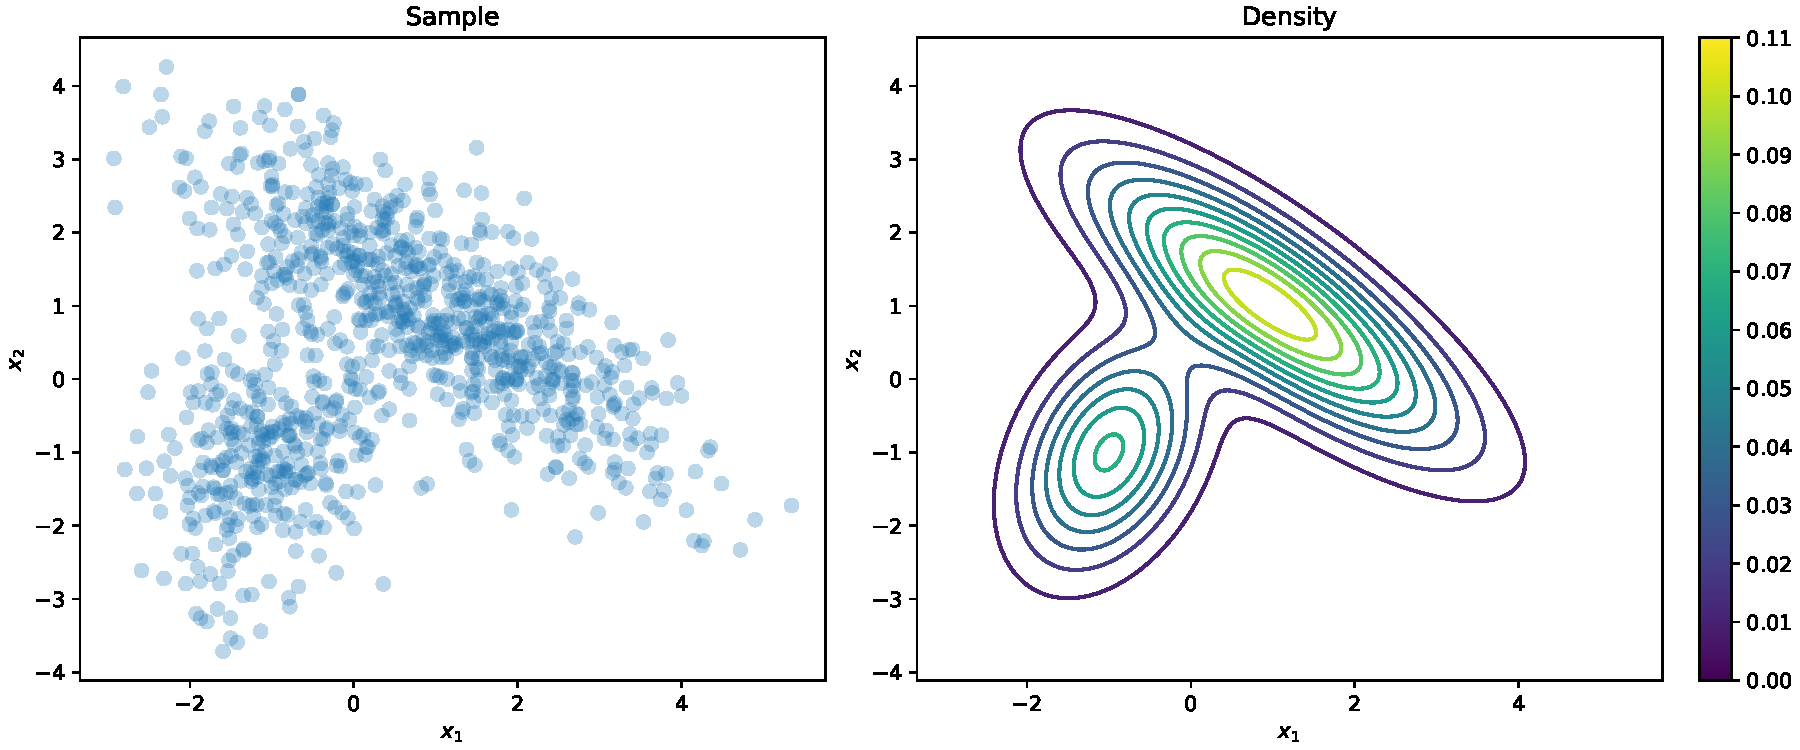
\includegraphics[width=1.0\textwidth]{gaussian-mixture-sample.pdf}
}
\caption{A sample from the bivariate Gaussian mixture with two components and its probability density.
\label{fig:gmm:sample}}
\end{figure}

\paragraph{Na\"ive thinning.} We select elements of the sample with uniformly spaced indices. Since the samples are i.i.d., na\"ive thinning is equivalent to drawing a smaller sample from the bivariate Gaussian mixture directly.

\paragraph{Stein thinning.} The gradients of the log-target required by the Stein thinning algorithm can be obtained analytically in this case (see Appendix~\ref{appendix:derivations:gaussian-mixture-gradient}).

\paragraph{Gradient-free Stein thinning.} This approach requires us to select an auxiliary distribution. We consider several options:
\begin{itemize}
\item a bivariate Gaussian with the mean and covariance matrix matching the sample mean and covariance of the sample (we call this approach ``simple Gaussian''),
\item a Laplace approximation of the target distribution (see Section 3.4 in \cite{robertMonteCarloStatistical2004}),
\item a KDE approximation of the target constructed from the sample (see, for example, Section 4.2 in \cite{ruppertStatisticsDataAnalysis2015}).
\end{itemize}

We use numerical optimisation provided by the function \texttt{scipy.\allowbreak optimize.\allowbreak minimize} in the Python library \texttt{scipy}\footnote{\url{https://scipy.org}} to find the mode of the log-target as well as the Hessian matrix evaluated at the mode, and construct the Laplace approximation.
For the KDE estimator, we use the Gaussian kernel, as implemented in the \texttt{scipy.\allowbreak stats.\allowbreak gaussian\_kde} function from the same library.

We evaluate the log-density of the chosen auxiliary distribution and the gradient for all sample points and use \Cref{alg:gf} to obtain a thinned sample. The results are shown in \Cref{fig:gmm:thinned}. The failure of the Laplace approximation is striking, so we investigate it further. The other methods produce visually sensible results.

\begin{figure}[h!]
\centering
\makebox[\textwidth][c]{
	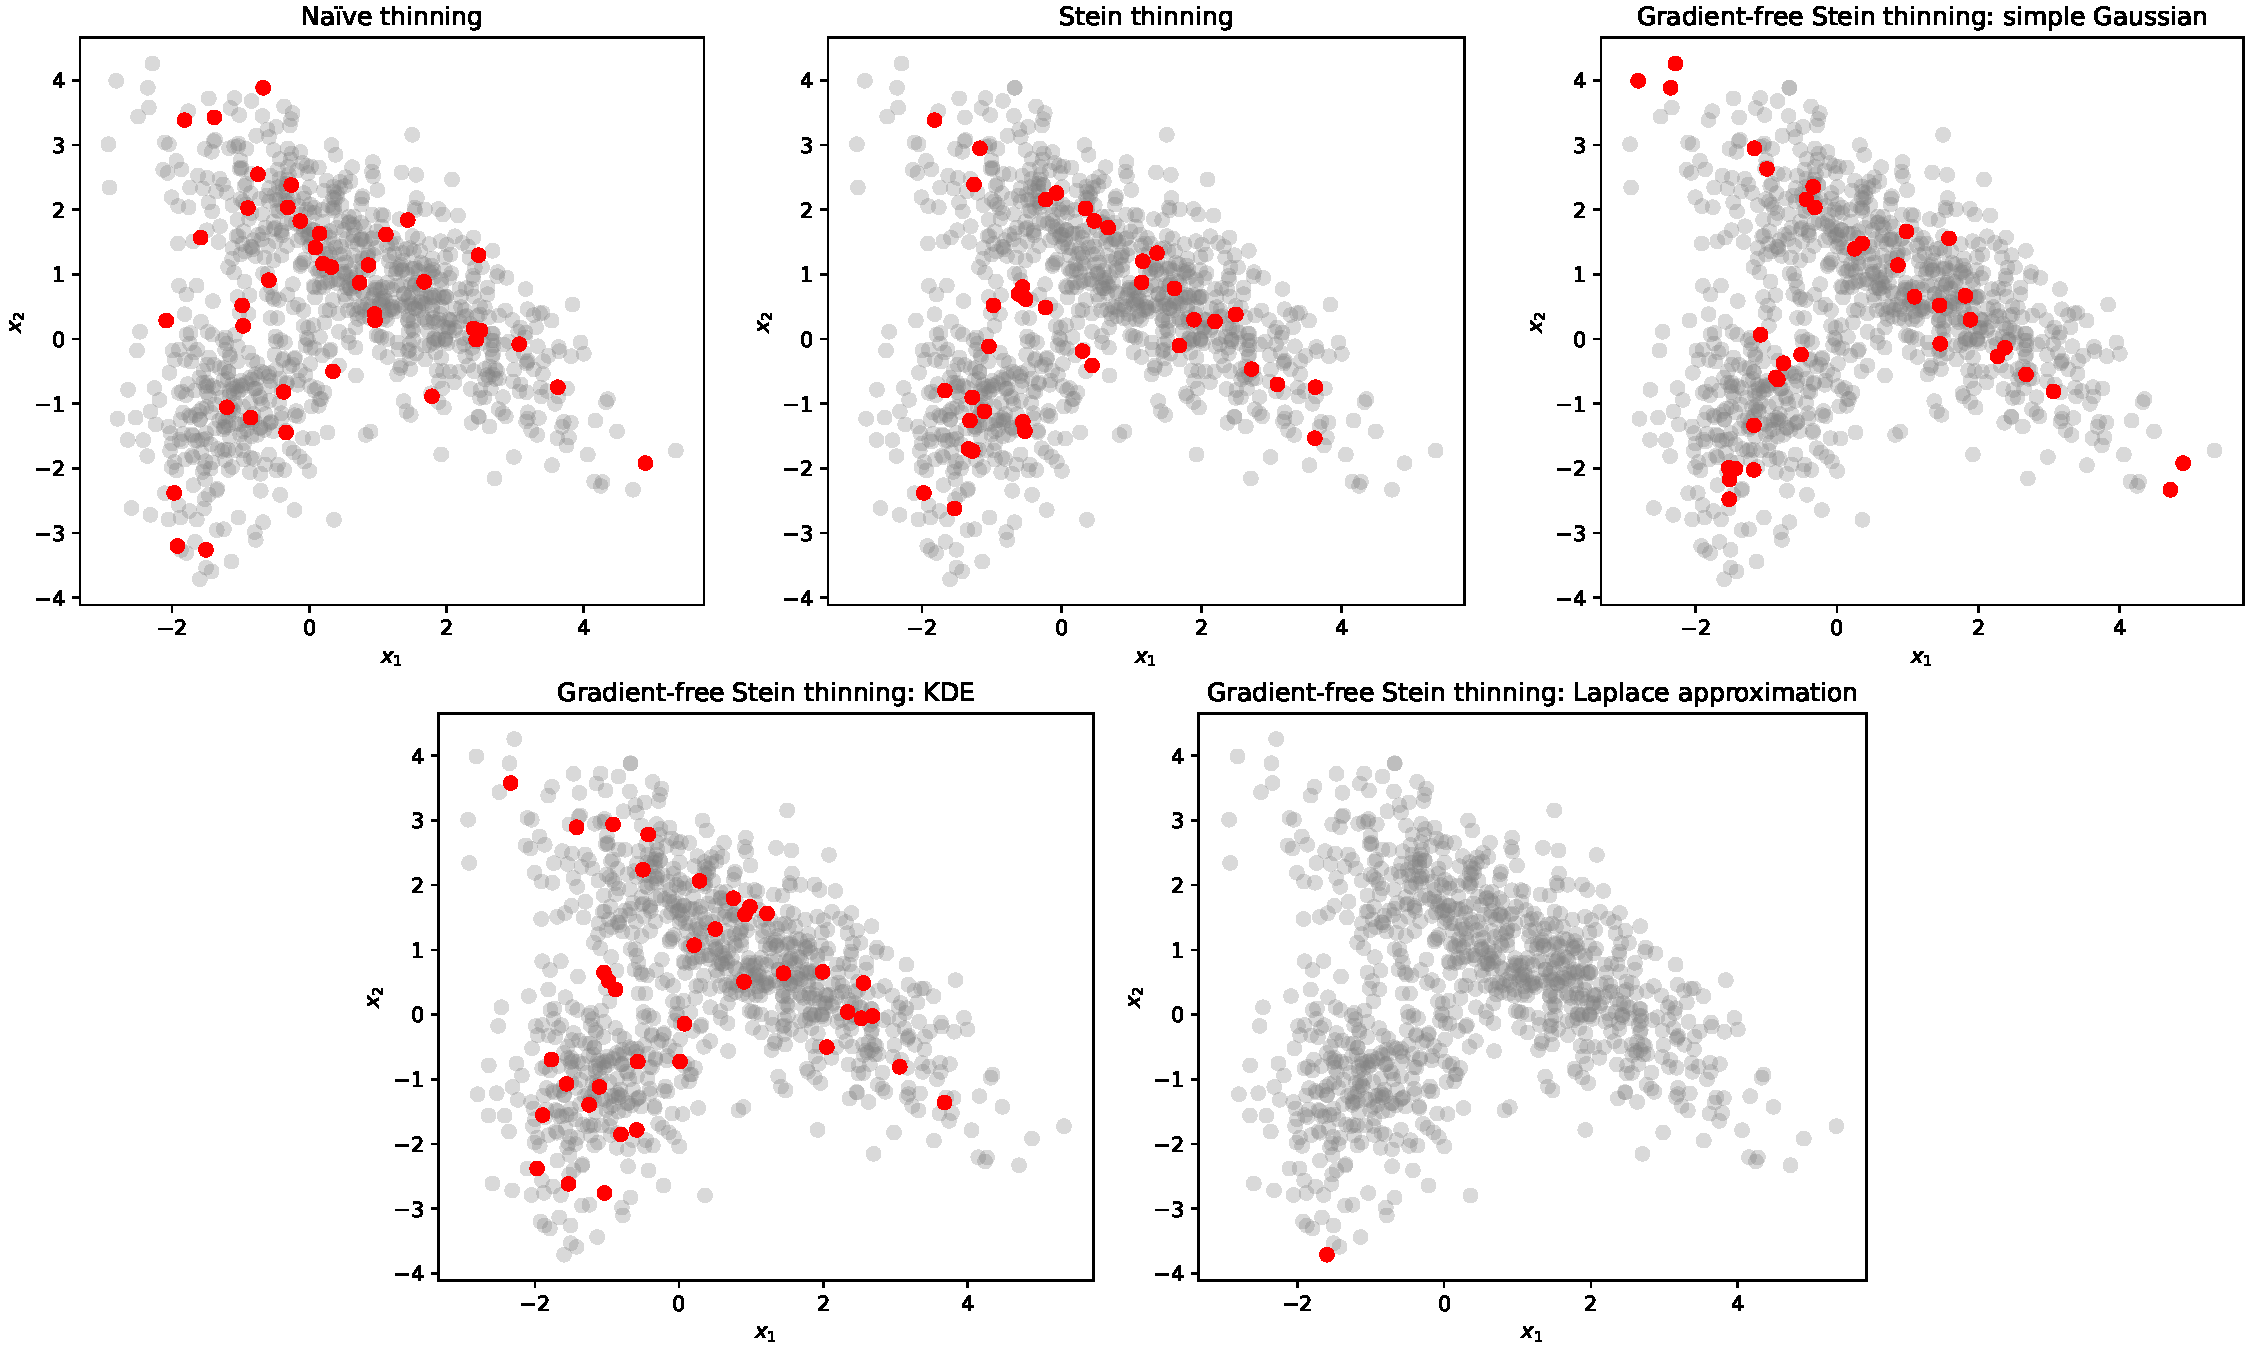
\includegraphics[width=1.0\textwidth]{gaussian-mixture-thinned-20.pdf}
}
\caption{Thinning results for the bivariate Gaussian mixture.
\label{fig:gmm:thinned}}
\end{figure}

To see why the Laplace approximation fails in this case, recall that~(\ref{eq:k_P_Q:expanded}) can be written in the form~(\ref{eq:k_P_Q}) and note the multiplier $q(x) / p(x)$. In \Cref{fig:gmm:laplace-failure}, we plot the values $\log_{10} q(x) - \log_{10} p(x) = \log_{10} (q(x) / p(x))$ for points in the sample, and \Cref{fig:gmm:kQ:hist} shows the histogram of $|k_Q(x_i, x_j)|$. We can see that $q(x) / p(x)$ varies by about 15 orders of magnitude, while $|k_Q(x_i, x_j)|$ varies only by about 8 orders of magnitude, therefore the scale of $q(x) / p(x)$ will tend to dominate the product
\begin{equation*}
\frac{q(x_i)}{p(x_i)} \frac{q(x_j)}{p(x_j)} k_Q(x_i, x_j),
\end{equation*}
especially for the diagonal elements
\begin{equation*}
\frac{q(x_i)}{p(x_i)} \frac{q(x_i)}{p(x_i)} k_Q(x_i, x_i).
\end{equation*}
\Cref{fig:gmm:laplace:first-iterations} in the Appendix confirms that the algorithm is compelled to select the same point as a result. By contrast, using the Gaussian distribution with the sample mean and covariance results in a considerably narrower range of $q(x) / p(x)$, as can be seen in \Cref{fig:gmm:laplace-failure}(b), allowing the algorithm to produce a thinned sample.

\begin{figure}[h]
\centering
\makebox[\textwidth][c]{
	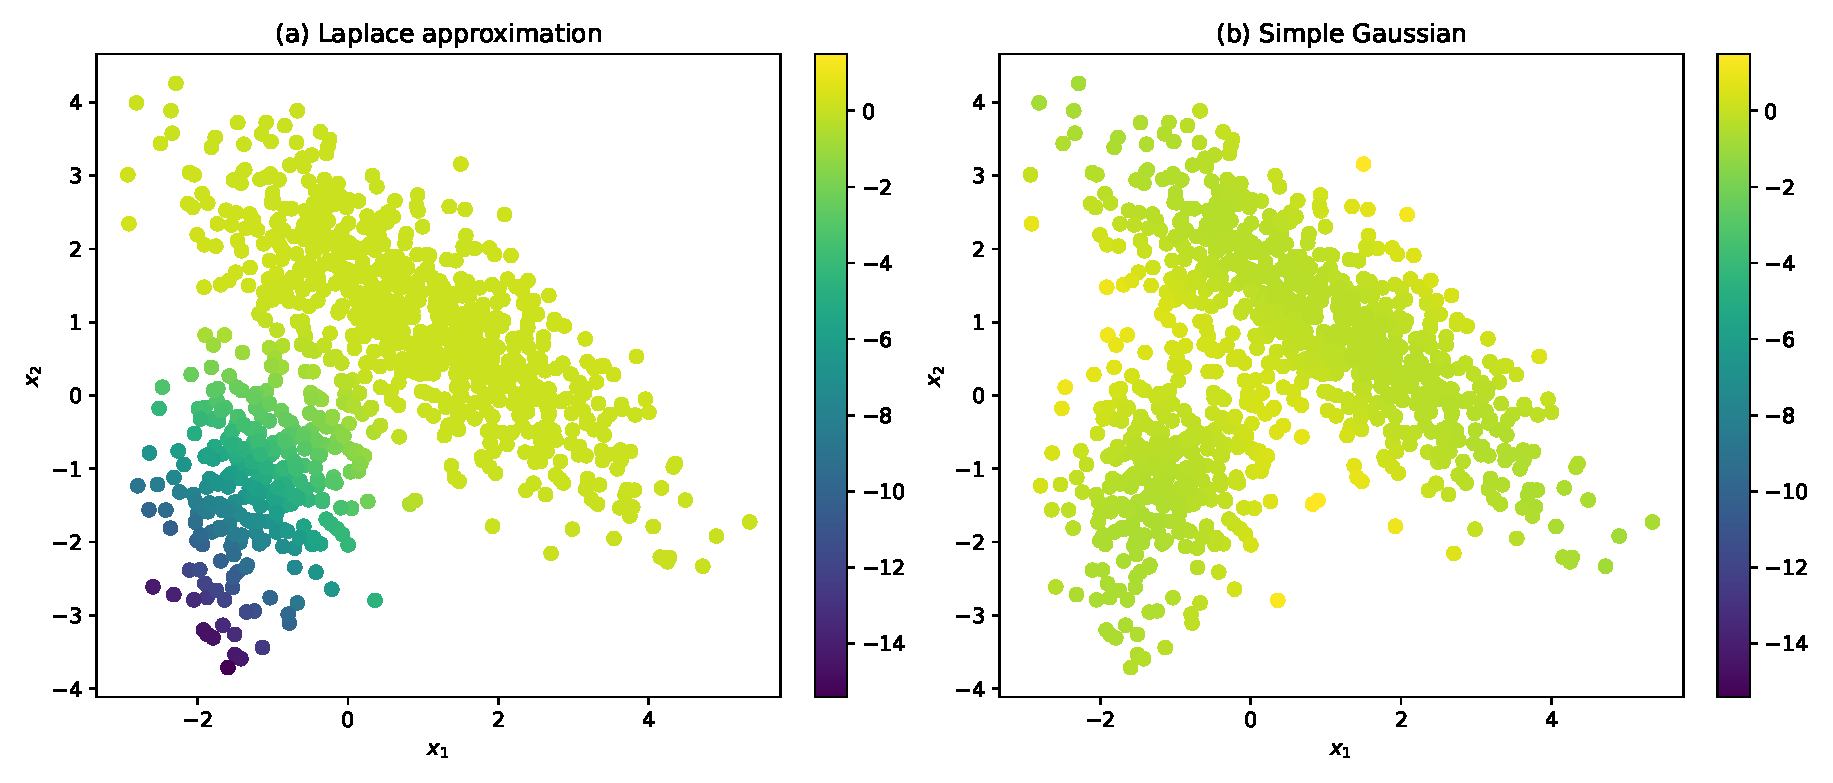
\includegraphics[width=1.0\textwidth]{gaussian-mixture-laplace-proxy.eps}
}
\caption{The values of $\log_{10} q(x) - \log_{10} p(x)$ for the points in the Gaussian mixture sample under (a)~the Laplace approximation and (b)~the simple Gaussian using the sample mean and covariance.
\label{fig:gmm:laplace-failure}}
\end{figure}

\begin{figure}[h]
\centering
\makebox[\textwidth][c]{
	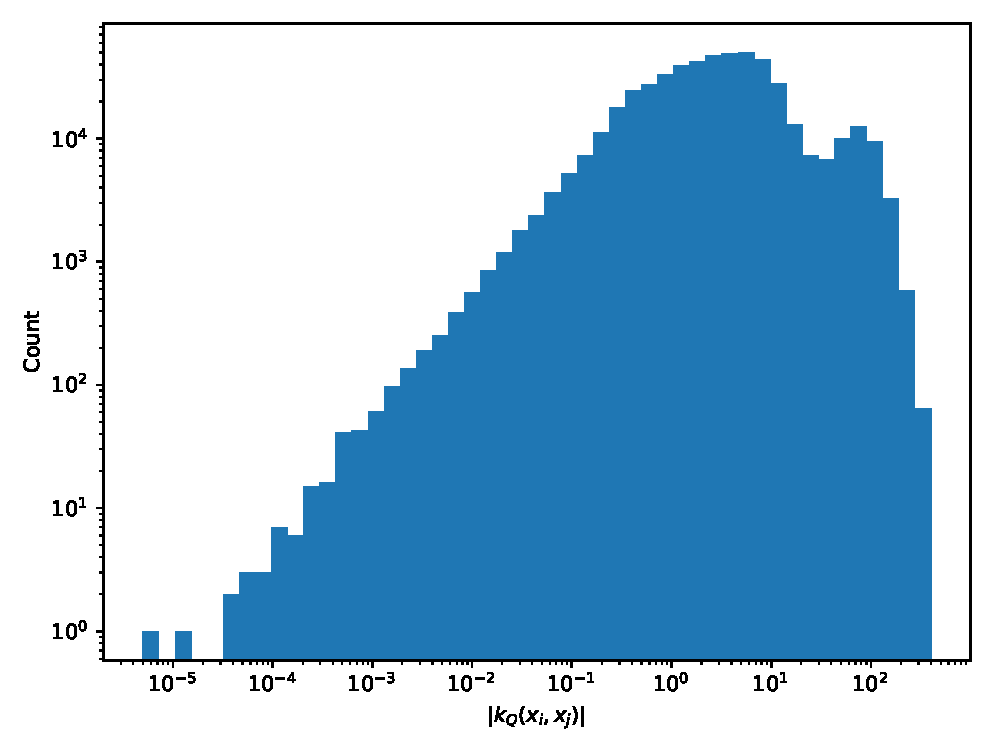
\includegraphics[width=0.5\textwidth]{gaussian-mixture-kQ-hist.eps}
}
\caption{Histogram of values $|k_Q(x_i, x_j)|$ for the bivariate Gaussian mixture using the Laplace approximation.
\label{fig:gmm:kQ:hist}}
\end{figure}

Finally, \Cref{fig:gmm:comparison} compares the energy distance achieved by thinned samples using the approaches above. The validation sample used in evaluating the energy distance is a separate i.i.d.\ sample of size 1000 from the same Gaussian mixture. We see that the gradient-free approach using the KDE is competitive with Stein thinning for small cardinalities, but loses out as the required sample size grows. Unsurprisingly, using the simple Gaussian approximation proves inferior to KDE.

\begin{figure}[h]
\centering
\makebox[\textwidth][c]{
	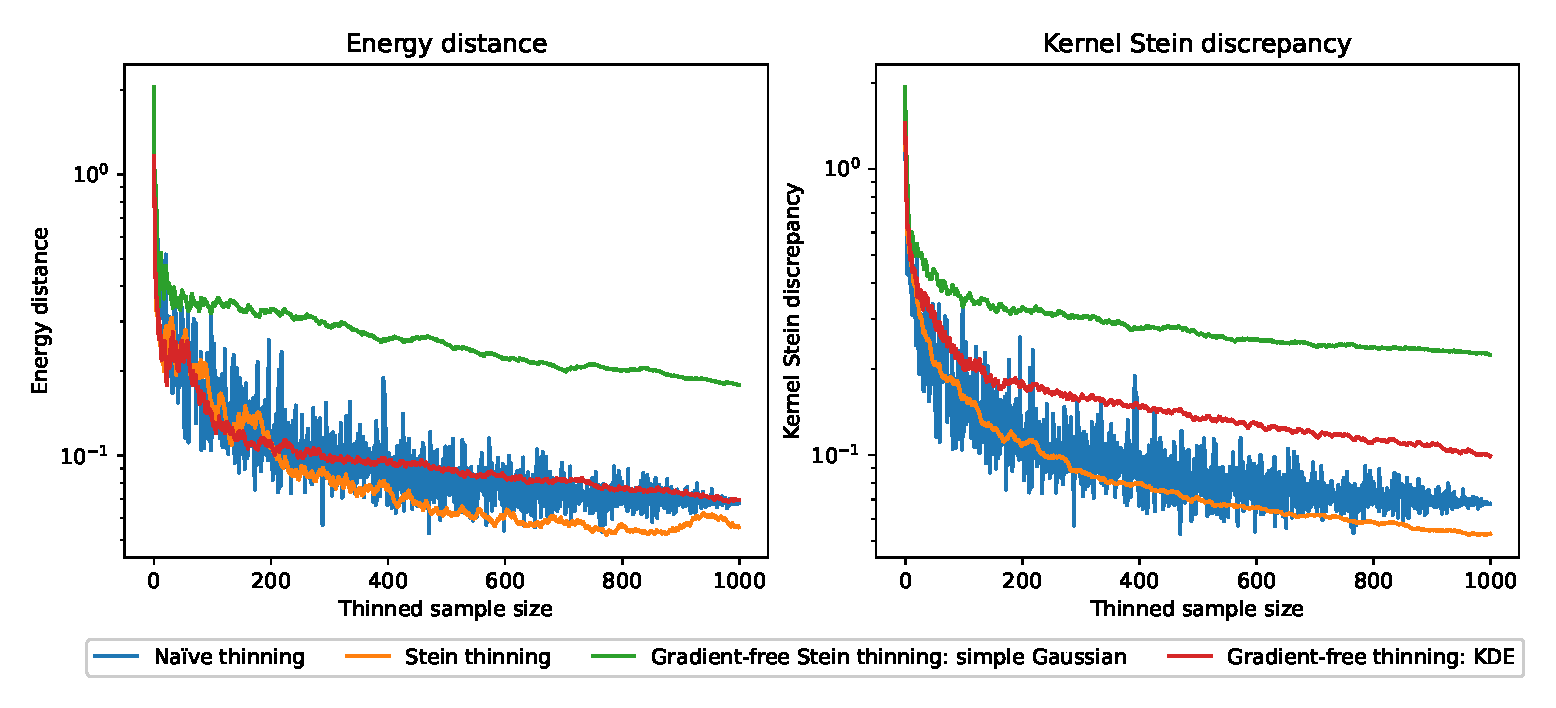
\includegraphics[width=1.0\textwidth]{gaussian-mixture-comparison.eps}
}
\caption{Comparison between thinning approaches for the bivariate Gaussian mixture sample.
\label{fig:gmm:comparison}}
\end{figure}

We conclude that even in such a favourable setup, the performance of the gradient-free algorithm depends crucially on the choice of the auxiliary distribution, which needs to provide an adequate enough approximation of the target.

\subsection{Lotka-Volterra inverse problem}
\label{sec:lotka-volterra}

A more challenging case is presented by the inverse problem of parameter inference for the Lotka-Volterra model, where the posterior cannot be sampled from directly, calling for a MCMC simulation, and thus bringing about the issue of burn-in.

The Lotka-Volterra model (\cite{lotkaElementsPhysicalBiology1925,volterraVariazioniFluttuazioniNumero1926}) describes the evolution of an idealised ecosystem with two species: predator and prey. The predator population grows while prey is abundant, and the prey population shrinks when there are too many predators. Denoting the size of prey population by $u_1$, and the predator population by $u_2$, the model postulates the following dynamic:
%\begin{equation}
%\begin{alignat*}{4}
%\frac{\diff u_1}{u_1} & = ( &  \theta_1 & & - \theta_2 u_2 & ) & & \diff t \\
%\frac{\diff u_2}{u_2} & = ( & -\theta_3 & & + \theta_4 u_1 & ) & & \diff t \\
%\end{alignat*}
%\end{equation}
\begin{equation}
\begin{aligned}
\frac{\diff u_1}{\diff t} & = \theta_1 u_1 - \theta_2 u_1 u_2, \\
\frac{\diff u_2}{\diff t} & = -\theta_3 u_2 + \theta_4 u_1 u_2, \\
\end{aligned}
\label{eq:lotka-volterra}
\end{equation}
with $\theta_1, \dots, \theta_4 > 0$. The resulting behaviour of the system is driven by the four parameters $\theta_1, \dots, \theta_4$. It is convenient to denote the solution to this system as  $u(t;\theta) = (u_1(t; \theta), u_2(t; \theta))^T$, where $\theta$ is the vector of parameter values $(\theta_1, \dots, \theta_4)^T$.

If a realisation of $u(t; \theta)$ is observed with noise for an interval $t \in [0, T]$ with $\theta$ unknown, one may wish to infer the values of the parameters that best describe the observed behaviour. In a practical setting, this corresponds to formulating a parametric model of a natural phenomenon and inferring the parameters of the model from the measurements of the phenomenon. We emulate this situation by fixing the true model, generating a realisation perturbed by noise and then attempting to recover the parameters of the true model from the realisation.

We take $u(t;\theta^*)$ to be generated for $t \in [0, 25]$ by the model~(\ref{eq:lotka-volterra}) with parameters $\theta^* = (0.67, 1.33, 1, 1)^T$ and initial value $u(0; \theta^*) = (1, 1)^T$. The interval $[0, 25]$ is discretised into $N = 2400$ points, so that $t_i = 25 \cdot i / (N - 1)$ for $i \in \{0, N - 1\}$. Bivariate i.i.d.\ Gaussian noise $\varepsilon(t) \sim \mathcal{N}\left( 0, \diag(0.2^2, 0.2^2) \right)$ is then added to all data points to emulate the measurement error, and we take the resulting time series $y(t) = u(t;\theta^*) + \varepsilon(t)$ as our observed data. \Cref{fig:lotka-volterra:data} displays the values $y(t)$. For comparability of results, the parameter values above match those used by \cite{riabizOptimalThinningMCMC2022}. 

\begin{figure}[h]
\centering
\makebox[\textwidth][c]{
	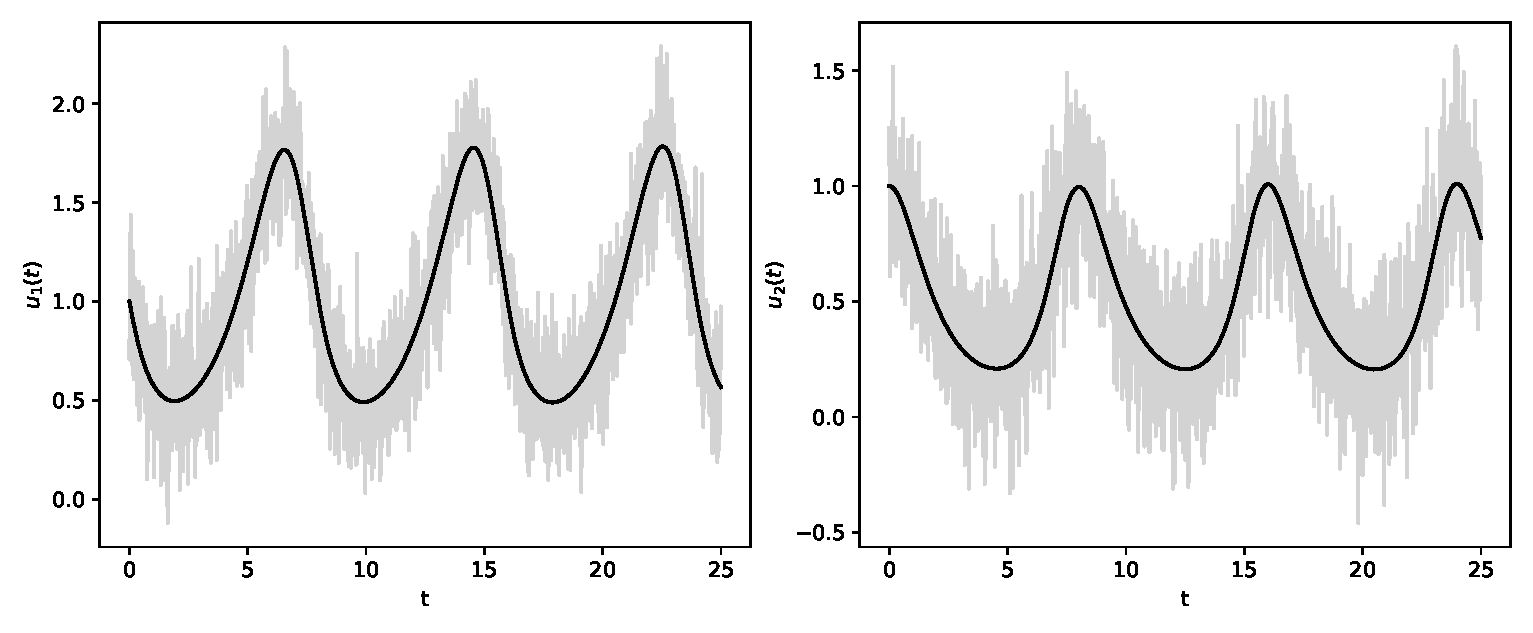
\includegraphics[width=1.0\textwidth]{lotka-volterra.eps}
}
\caption{Solution to the Lotka-Volterra ODEs (black) with added Gaussian noise (grey).
\label{fig:lotka-volterra:data}}
\end{figure}

Posterior inference is then performed by means of a random-walk Metropolis-Hastings algorithm. Assuming independent observations, we take the likelihood to be
\begin{equation}
\mathcal{L}(\theta) = \prod_{i=1}^N \phi_i(u(t_i; \theta)),
\label{eq:lotka-volterra:likelihood}
\end{equation}
where 
\begin{equation}
\phi_i(u(t_i;\theta)) \propto \exp\left( -\frac{1}{2} (y(t_i) - u(t_i; \theta))^T C^{-1} (y(t_i) - u(t_i; \theta)) \right)
\label{eq:lotka-volterra:error-distr}
\end{equation}
with $C = \diag(0.2^2, 0.2^2)$. Since $\theta_i > 0$, we put independent log-normal priors on each $\theta_i$, so
\begin{equation}
\pi(\theta) \propto \exp \left(-\frac{1}{2} (\log \theta)^T (\log \theta) \right),
\label{eq:lotka-volterra:prior}
\end{equation}
where the logarithm in $\log \theta$ is applied component-wise.
By the Bayes theorem, the posterior is then
\begin{equation}
p(\theta) \propto \mathcal{L}(\theta) \pi(\theta).
\label{eq:lotka-volterra:posterior}
\end{equation}
We follow \cite{riabizOptimalThinningMCMC2022} in selecting the starting values for the chains, given in Table~\ref{table:lotka-volterra:starting_values}.

\begin{table}[h!]
\centering
\begin{tabularx}{0.5\textwidth}{c Y Y Y Y} 
 \hline
 Chain & $\theta_1$ & $\theta_2$ & $\theta_3$ & $\theta_4$ \\
 \hline
 1 & 0.55 & 1    & 0.8 & 0.8 \\ 
 2 & 1.5  & 1    & 0.8 & 0.8 \\
 3 & 1.3  & 1.33 & 0.5 & 0.8 \\
 4 & 0.55 & 3    & 3.  & 0.8 \\
 5 & 0.55 & 1    & 1.5 & 1.5 \\
 \hline
\end{tabularx}
\caption{Starting values for the random-walk Metropolis-Hastings algorithm for the Lotka-Volterra inverse problem.}
\label{table:lotka-volterra:starting_values}
\end{table}

Since the parameters $\theta$ of the Lotka-Volterra model are positive, we run MCMC in the log-space by applying the reparameterisation $\zeta_i = \log \theta_i$. The trace plots from 500,000 iterations of the random-walk Metropolis-Hastings algorithm for each chain are shown in \Cref{fig:lotka-volterra:trace-plots} in the Appendix. \Cref{fig:lotka-volterra:chain-paths} confirms that all chains reach the high-probability region, albeit after considerable burn-in, and \Cref{fig:lotka-volterra:chain1-sample} demonstrates the sample obtained from the first chain. Having obtained samples from the posterior distribution, we proceed to thin them.

\begin{figure}[h]
\centering
\makebox[\textwidth][c]{
	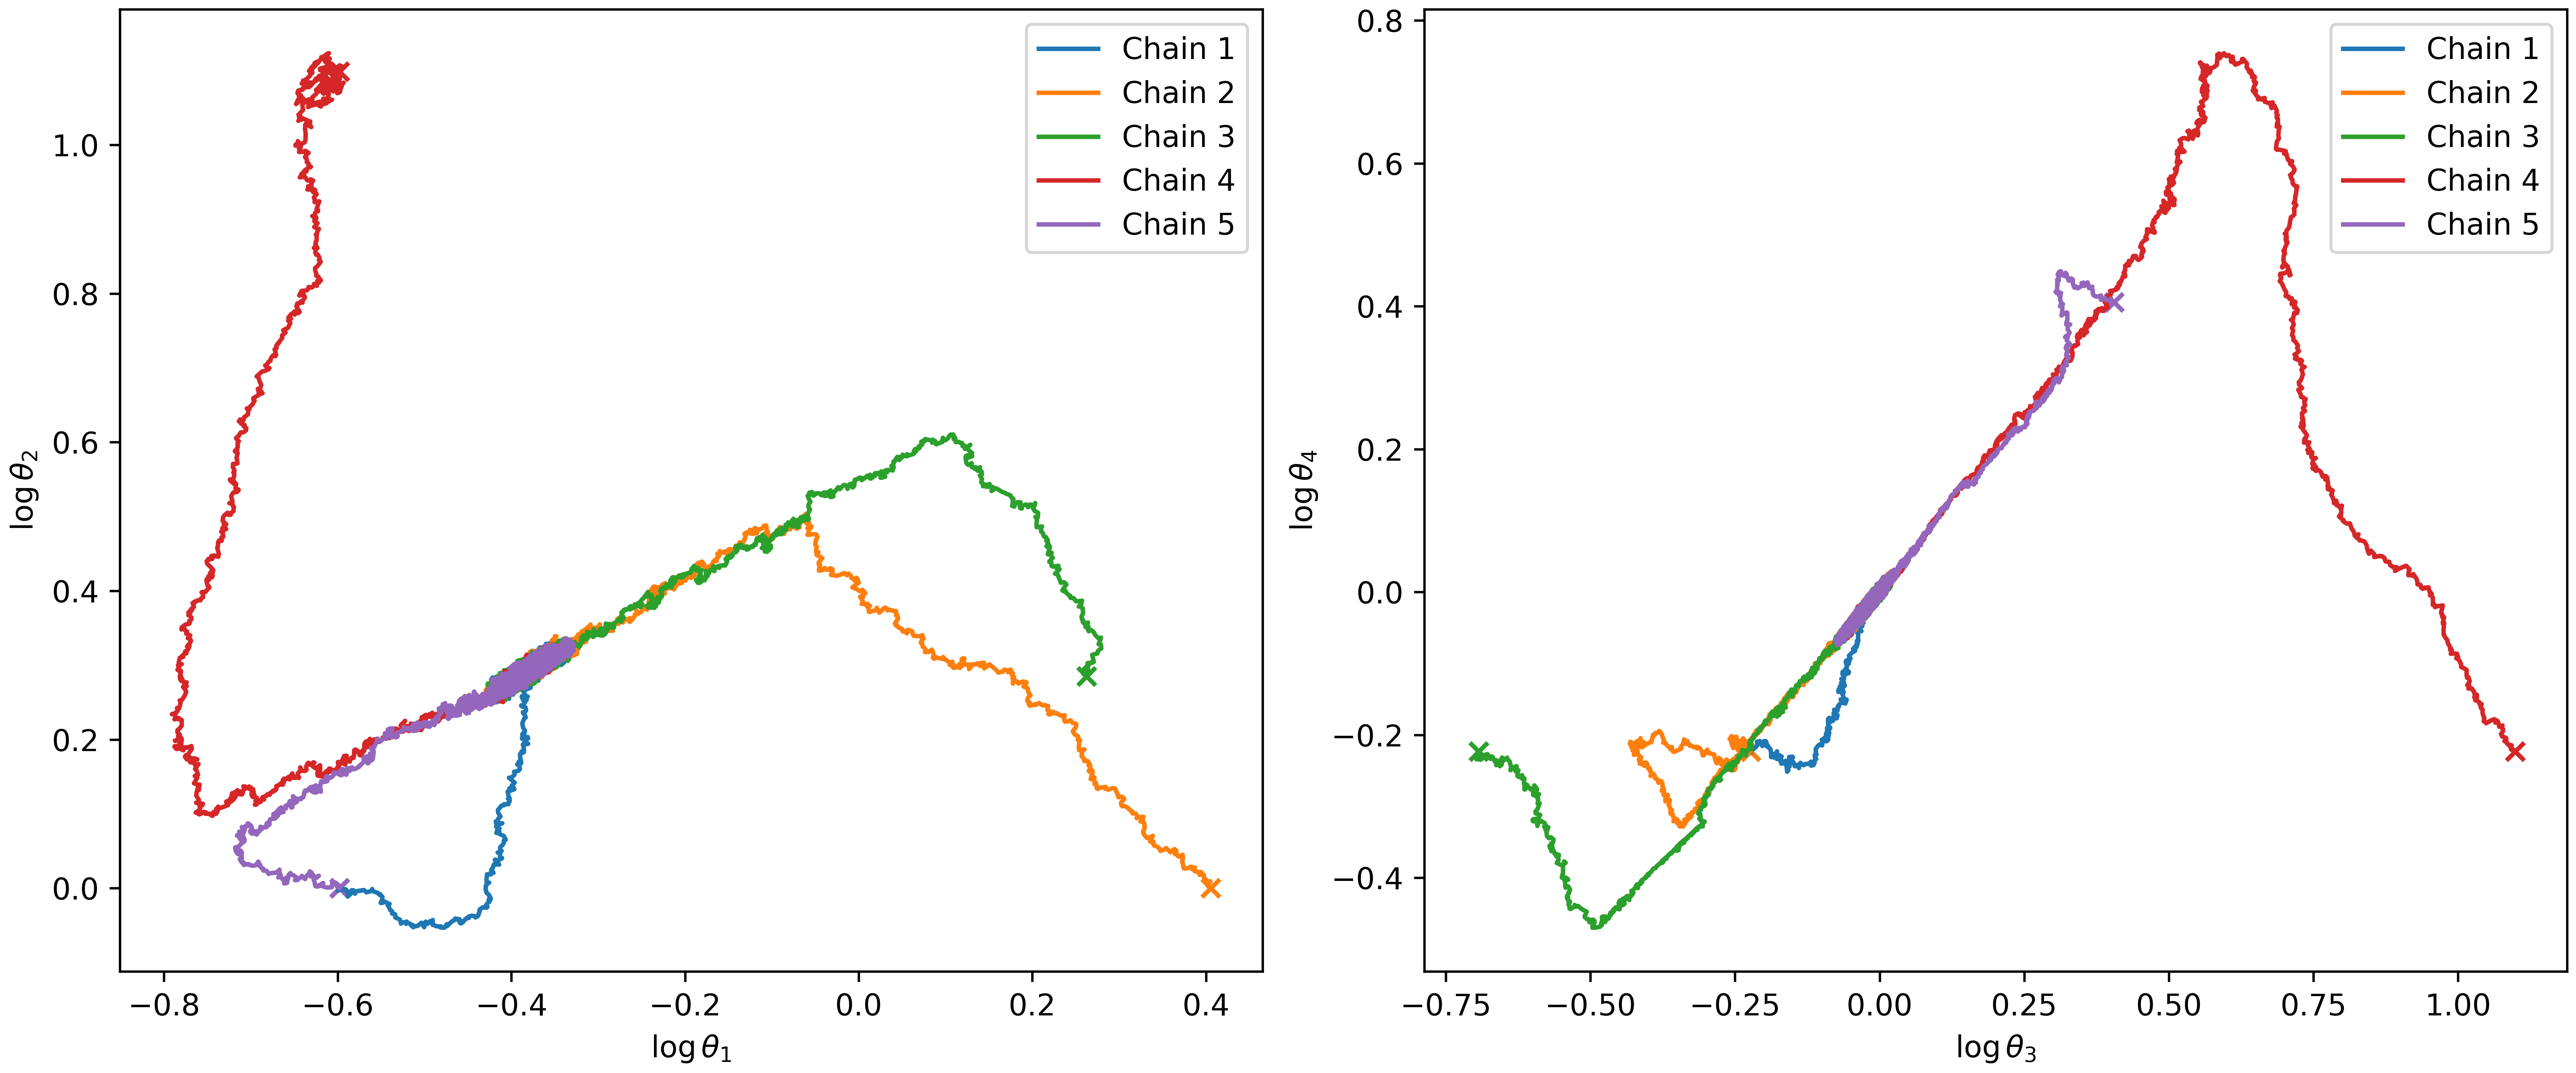
\includegraphics[width=1.0\textwidth]{lotka-volterra-chain-paths.png}
}
\caption{Projections of chain paths from the random-walk Metropolis-Hastings algorithm for the Lotka-Volterra inverse problem.
\label{fig:lotka-volterra:chain-paths}}
\end{figure}

\begin{figure}[h]
\centering
\makebox[\textwidth][c]{
	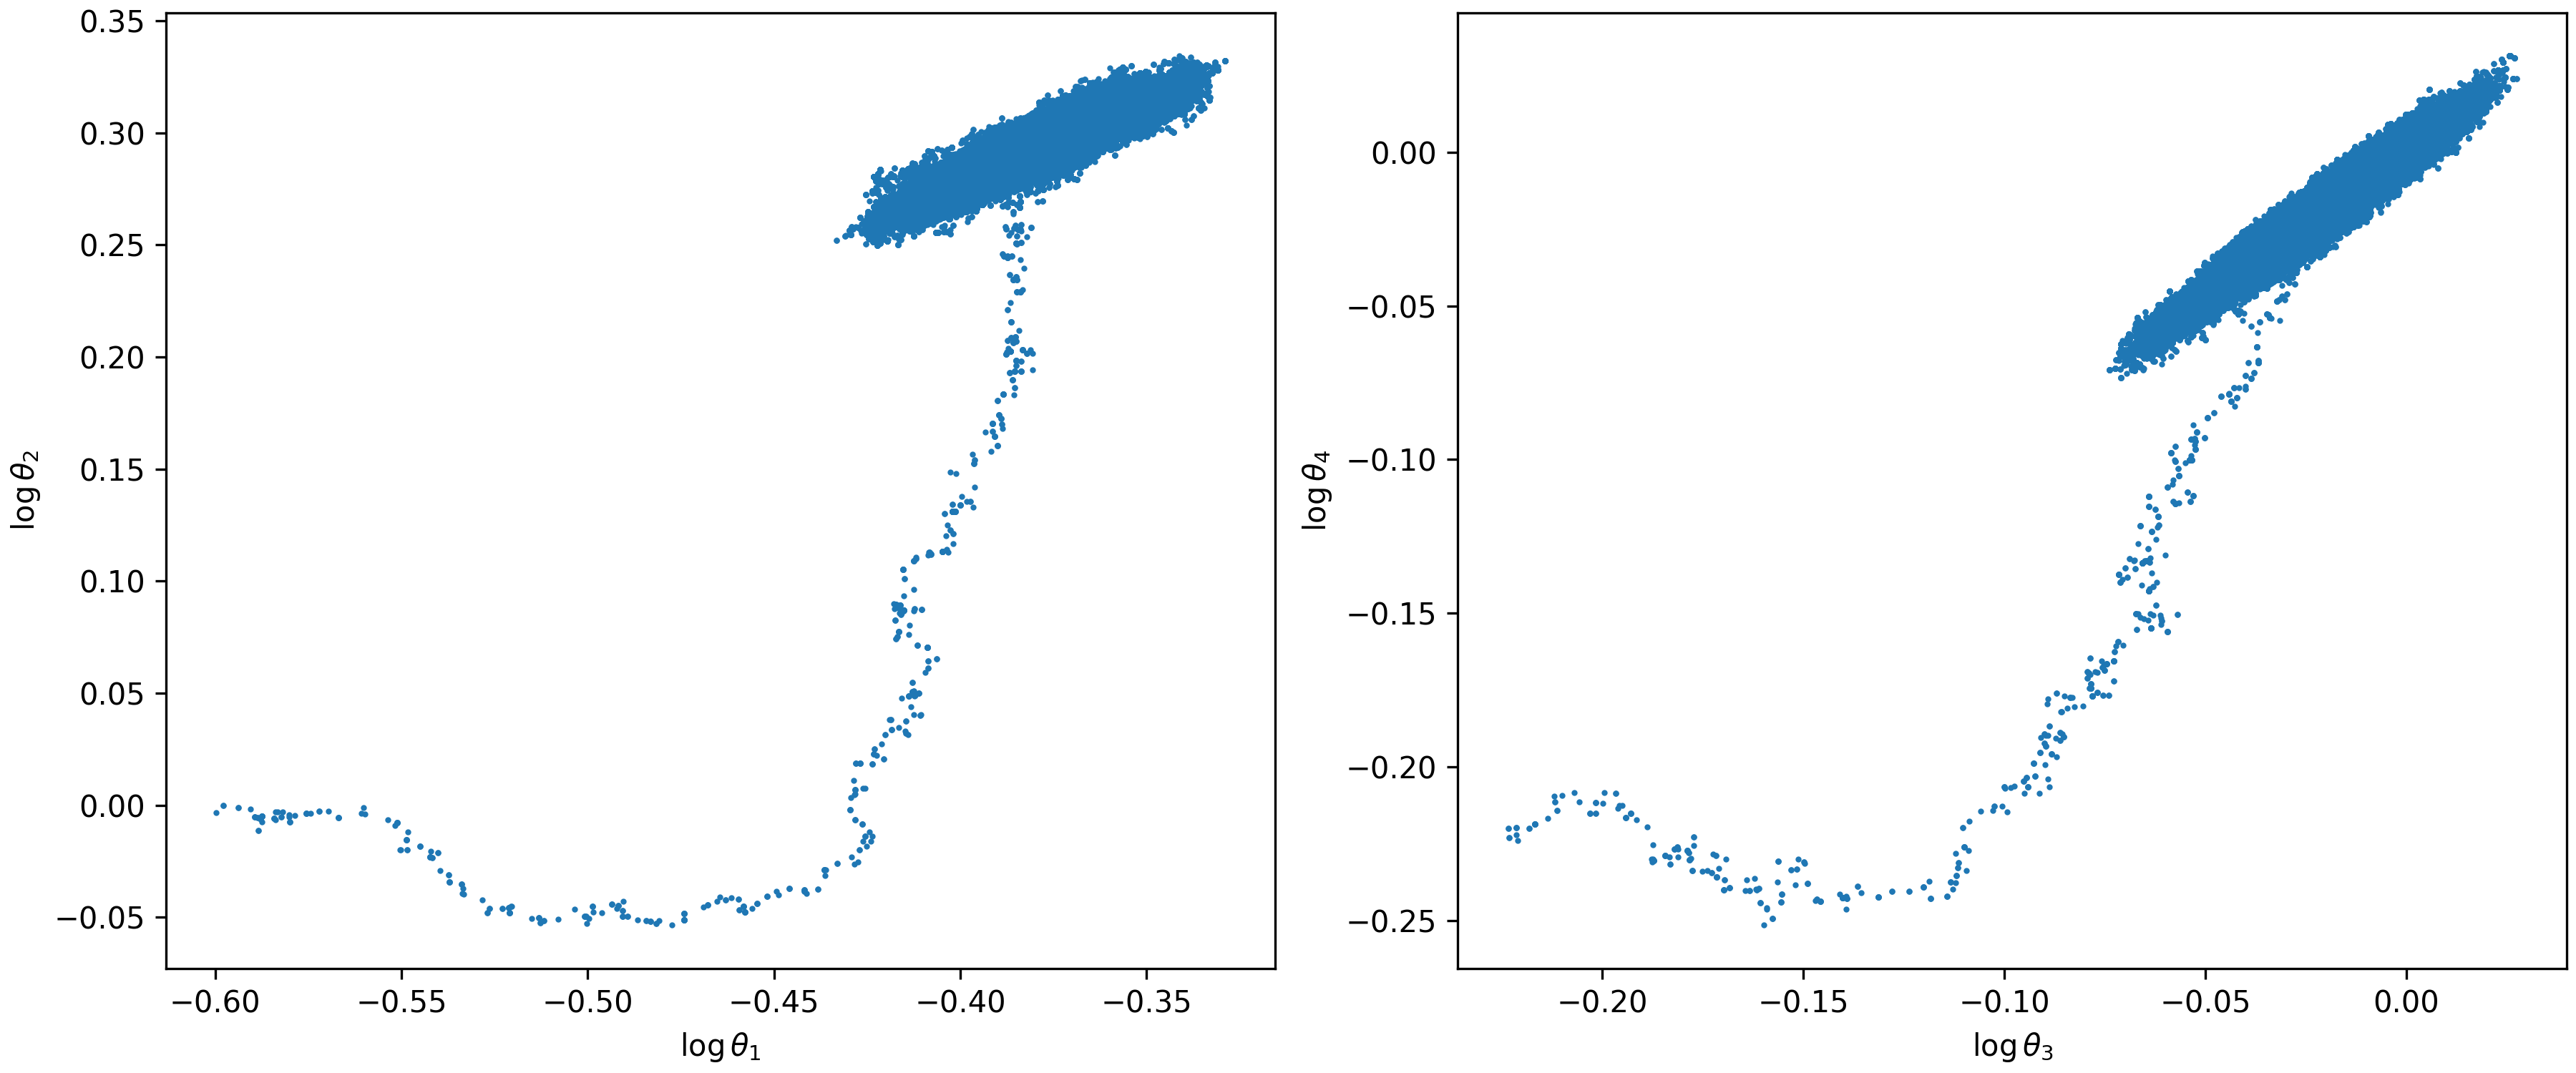
\includegraphics[width=1.0\textwidth]{lotka-volterra-chain1-sample.png}
}
\caption{Sample obtained from the first chain in the MCMC run for the Lotka-Volterra inverse problem.
\label{fig:lotka-volterra:chain1-sample}}
\end{figure}

\paragraph{Na\"ive thinning.} We select elements of the sample with uniformly spaced indices. The results are shown in \Cref{fig:lotka-volterra:naive:results} in the Appendix.

\paragraph{Stein thinning.} In order to use this approach, we need the gradients of the log-posterior density. From~(\ref{eq:lotka-volterra:posterior}), we have
\begin{equation*}
\nabla_{\theta} \log p(\theta) = \nabla_{\theta} \log \mathcal{L}(\theta) + \nabla_{\theta} \pi(\theta).
\end{equation*}
Equation~(\ref{eq:lotka-volterra:likelihood}) yields
\begin{equation*}
\frac{\partial}{\partial \theta_s} \log \mathcal{L}(\theta) 
= \sum_{i=1}^N \frac{\partial}{\partial \theta_s} \log \phi_i(u(t_i; \theta))
= \sum_{i=1}^N \sum_{r=1}^q \frac{\partial}{\partial u_r} (\log \phi_i) \frac{\partial u_r}{\partial \theta_s},
\end{equation*}
where $q = 2$ is the dimension of the vector $u(t)$ and $s \in \{1, \dots, 4\}$ indexes the components of $\theta$. This can be written in the matrix form as
\begin{equation*}
(\nabla_{\theta} \log \mathcal{L})(\theta) = \sum_{i=1}^N (S(t_i))^T (\nabla_{u} \log \phi_i)(u(t_i; \theta)),
\end{equation*}
where the elements of the sensitivities matrix are given by
\begin{equation*}
S_{r,s} \coloneq \frac{\partial u_r}{\partial \theta_s}
\end{equation*}
for $r \in \{1, 2\}$ and $s \in \{1, \dots, 4\}$.
The gradient
\begin{equation*}
(\nabla_u \log \phi_i)(u(t_i; \theta)) = C^{-1}(y(t_i) - u(t_i; \theta))
\end{equation*}
is derived directly from~(\ref{eq:lotka-volterra:error-distr}). In order to obtain the sensitivities $\partial u_r / \partial \theta_s$, we augment the system~(\ref{eq:lotka-volterra}) with additional forward sensitivity equations and solve it numerically. The derivation of the sensitivity equations can be found in Appendix~\ref{appendix:derivations:forward-sensitivity}. Alternatively, the sensitivities can be obtained by numerical differentiation, for example using the Python library \texttt{JAX}\footnote{\url{https://jax.readthedocs.io}}. Since the gradient is calculated independently for each element of the sample, these calculations can easily be parallelised at postprocessing stage\footnote{Parallelisation can be implemented with minimal effort using the Python \texttt{Dask} library (\url{https://docs.dask.org}) and run either locally or on Amazon Web Services (\url{https://aws.amazon.com}). See \url{https://github.com/aglebov/gradient-free-mcmc-postprocessing/blob/main/code/examples/Dask_AWS.ipynb} for a demonstration.}.

The gradient of the log-prior is obtained immediately from~(\ref{eq:lotka-volterra:prior}):
\begin{equation*}
\nabla_{\theta} \log \pi(\theta) = -\frac{\log \theta}{\theta},
\end{equation*}
where the logarithm and division are component-wise.

We have a choice of applying Stein thinning either in the linear or in the log-space of parameters. Note that this choice is separate from the choice of parameterisation for the MCMC run. By the chain rule when $\zeta_i = \log \theta_i$ we obtain
\begin{equation*}
\nabla_\zeta \log p(\zeta) = J^{-T} \nabla_\theta \log p(\theta),
\end{equation*}
where the Jacobian is $J = \text{diag}(\theta_1^{-1}, \dots, \theta_d^{-1})$, so $J^{-T} =  \text{diag}(\theta_1, \dots, \theta_d)$.
\Cref{fig:lotka-volterra:stein-thinning:energy-distance} shows that there is no discernible difference between the two options in terms of the resulting energy distance to the target distribution, so we use the logarithmic parameterisation in subsequent analysis. The first 20 points selected by Stein thinning are shown in \Cref{fig:lotka-volterra:stein:results} in the Appendix.

Comparing the performance of Stein thinning against na\"ive thinning (\Cref{fig:lotka-volterra:stein-thinning:energy-distance}), we observe that Stein thinning performs consistently for all chains, whereas na\"ive thinning fails for chain 4, which spent most of its time away from the high-probability region. Moreover, Stein thinning improves on na\"ive thinning for thinned sample sizes below 20 and above 2000 for all chains, and is otherwise similar.

\begin{figure}[h]
\centering
\makebox[\textwidth][c]{
	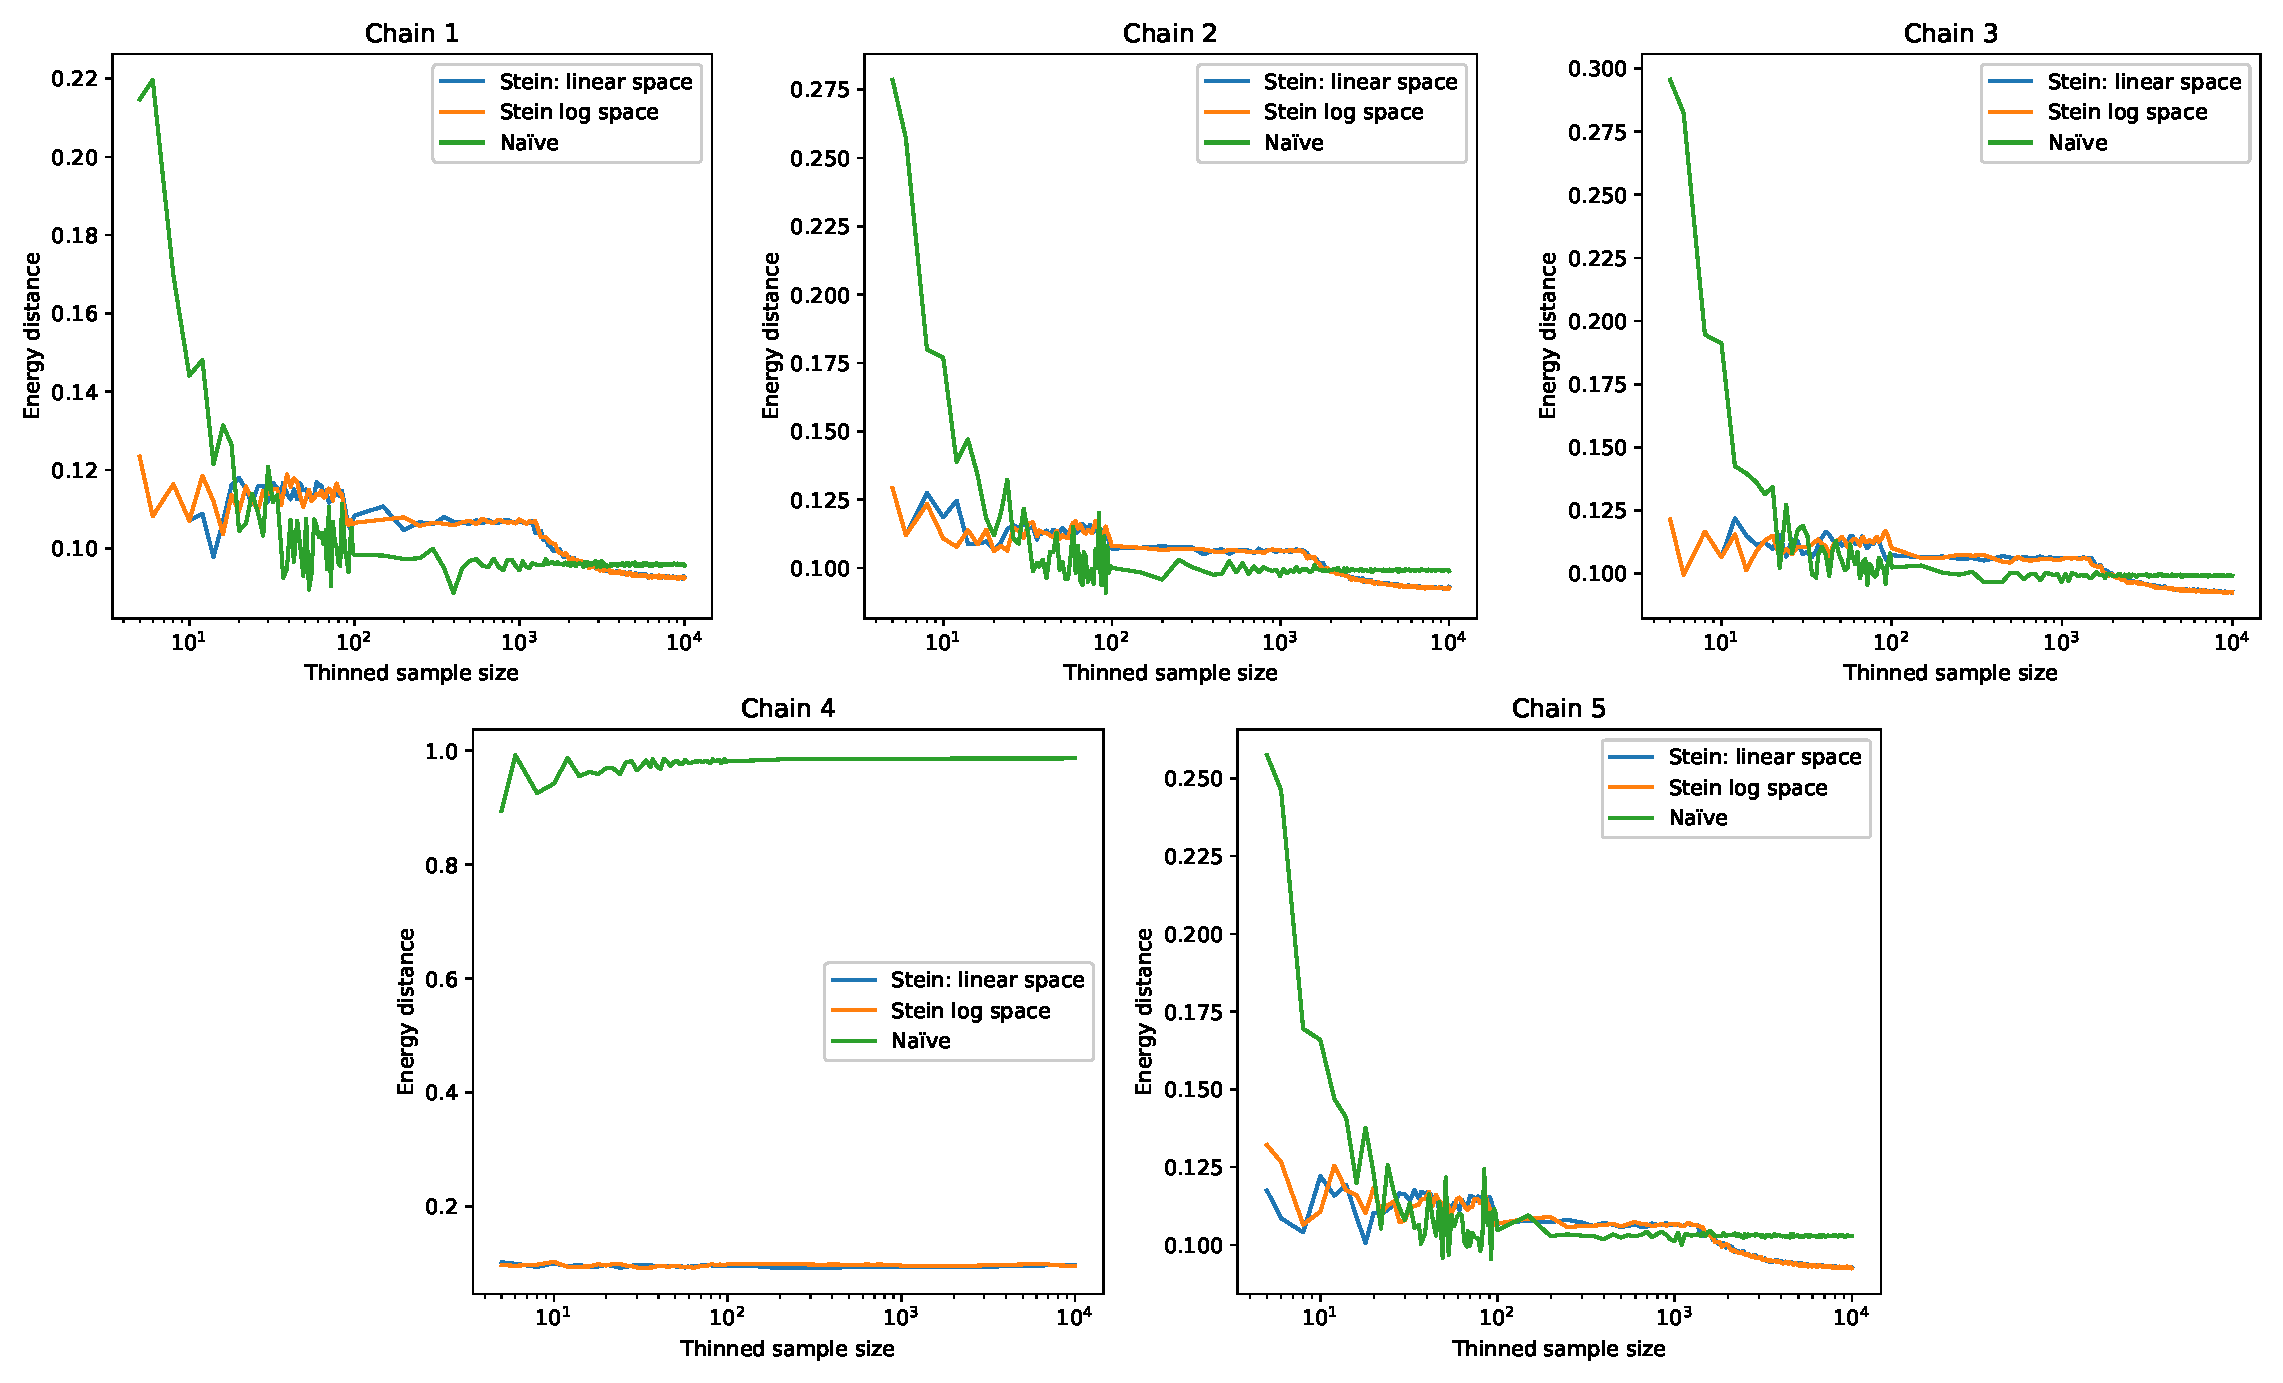
\includegraphics[width=1.0\textwidth]{lotka-volterra-stein-thinning-energy-distance.eps}
}
\caption{Energy distance comparison between Stein thinning (in linear and logarithmic space) and na\"ive thinning for MCMC chains in the Lotka-Volterra inverse problem.
\label{fig:lotka-volterra:stein-thinning:energy-distance}}
\end{figure}

The validation sample we use for calculating the energy distance in this case was obtained by running the HMC algorithm as implemented in the \texttt{PyStan}\footnote{\url{https://pystan.readthedocs.io}} library for 10,000 steps with the starting points shown in \Cref{table:lotka-volterra:starting_values} and concatenating the results for the five chains.

\paragraph{Gradient-free Stein thinning.} The choice of KDE as the auxiliary distribution, which performed best for the Gaussian mixture in \Cref{sec:gaussian-mixture}, becomes computationally infeasible here due to the size of the sample. Indeed, KDE places a kernel at the location of each sample point, so the cost of evaluating the resulting density once is $O(n)$, where $n$ is the sample size, since contributions from all kernels need to be added. \Cref{alg:gf} requires density estimates for each element of the sample, thus the total computational cost grows as $O(n^2)$ and becomes prohibitive for large samples. An alternative could be to place KDE kernels at a subset of points from the sample, however selecting such a subset is equivalent to the problem that thinning is trying to solve in the first place.

As in the case of the Gaussian mixture, the Laplace approximation fails to produce a thinned sample here due to ratio $q(x) / p(x)$ vanishing away from the mode, so we turn to a multivariate Gaussian with the mean and covariance matching the sample mean and covariance (``simple Gaussian''). \Cref{fig:lotka-volterra:gf-thinning:energy-distance} shows that the gradient-free approach is competitive with standard Stein thinning for chains 2-5 in terms of the resulting energy distance metric, but performs worse for the first chain. Most encouragingly, the gradient-free approach handles the sample from chain 4 well.

\begin{figure}[h]
\centering
\makebox[\textwidth][c]{
	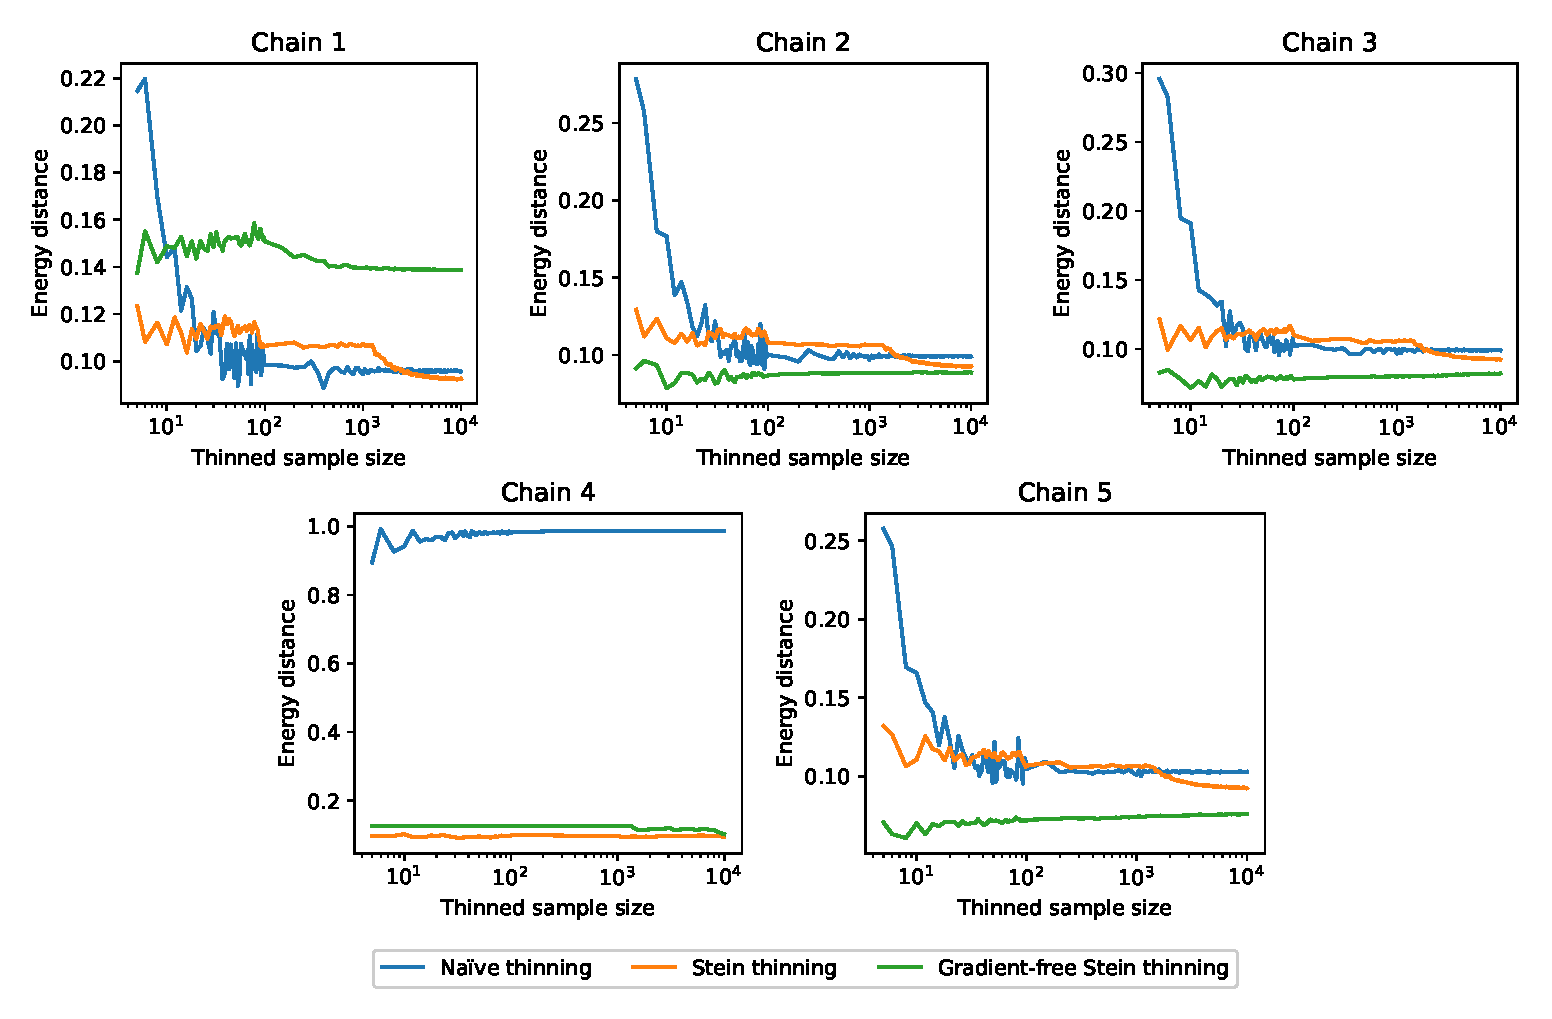
\includegraphics[width=1.0\textwidth]{lotka-volterra-gf-thinning-energy-distance.eps}
}
\caption{Energy distance comparison between gradient-free and standard Stein thinning for the Lotka-Volterra inverse problem.
\label{fig:lotka-volterra:gf-thinning:energy-distance}}
\end{figure}

It is perhaps surprising that gradient-free thinning, being an approximation, achieves lower values of energy distance compared to the gradient-based approach. Note, however, that the energy distance is not equivalent to KSD, and the two metrics are not in general minimised by the same sample. \Cref{fig:lotka-volterra:gf-thinning:ksd} confirms that the gradient-based algorithm consistently achieves the lowest values of KSD among the approaches considered.

\begin{figure}[h]
\centering
\makebox[\textwidth][c]{
	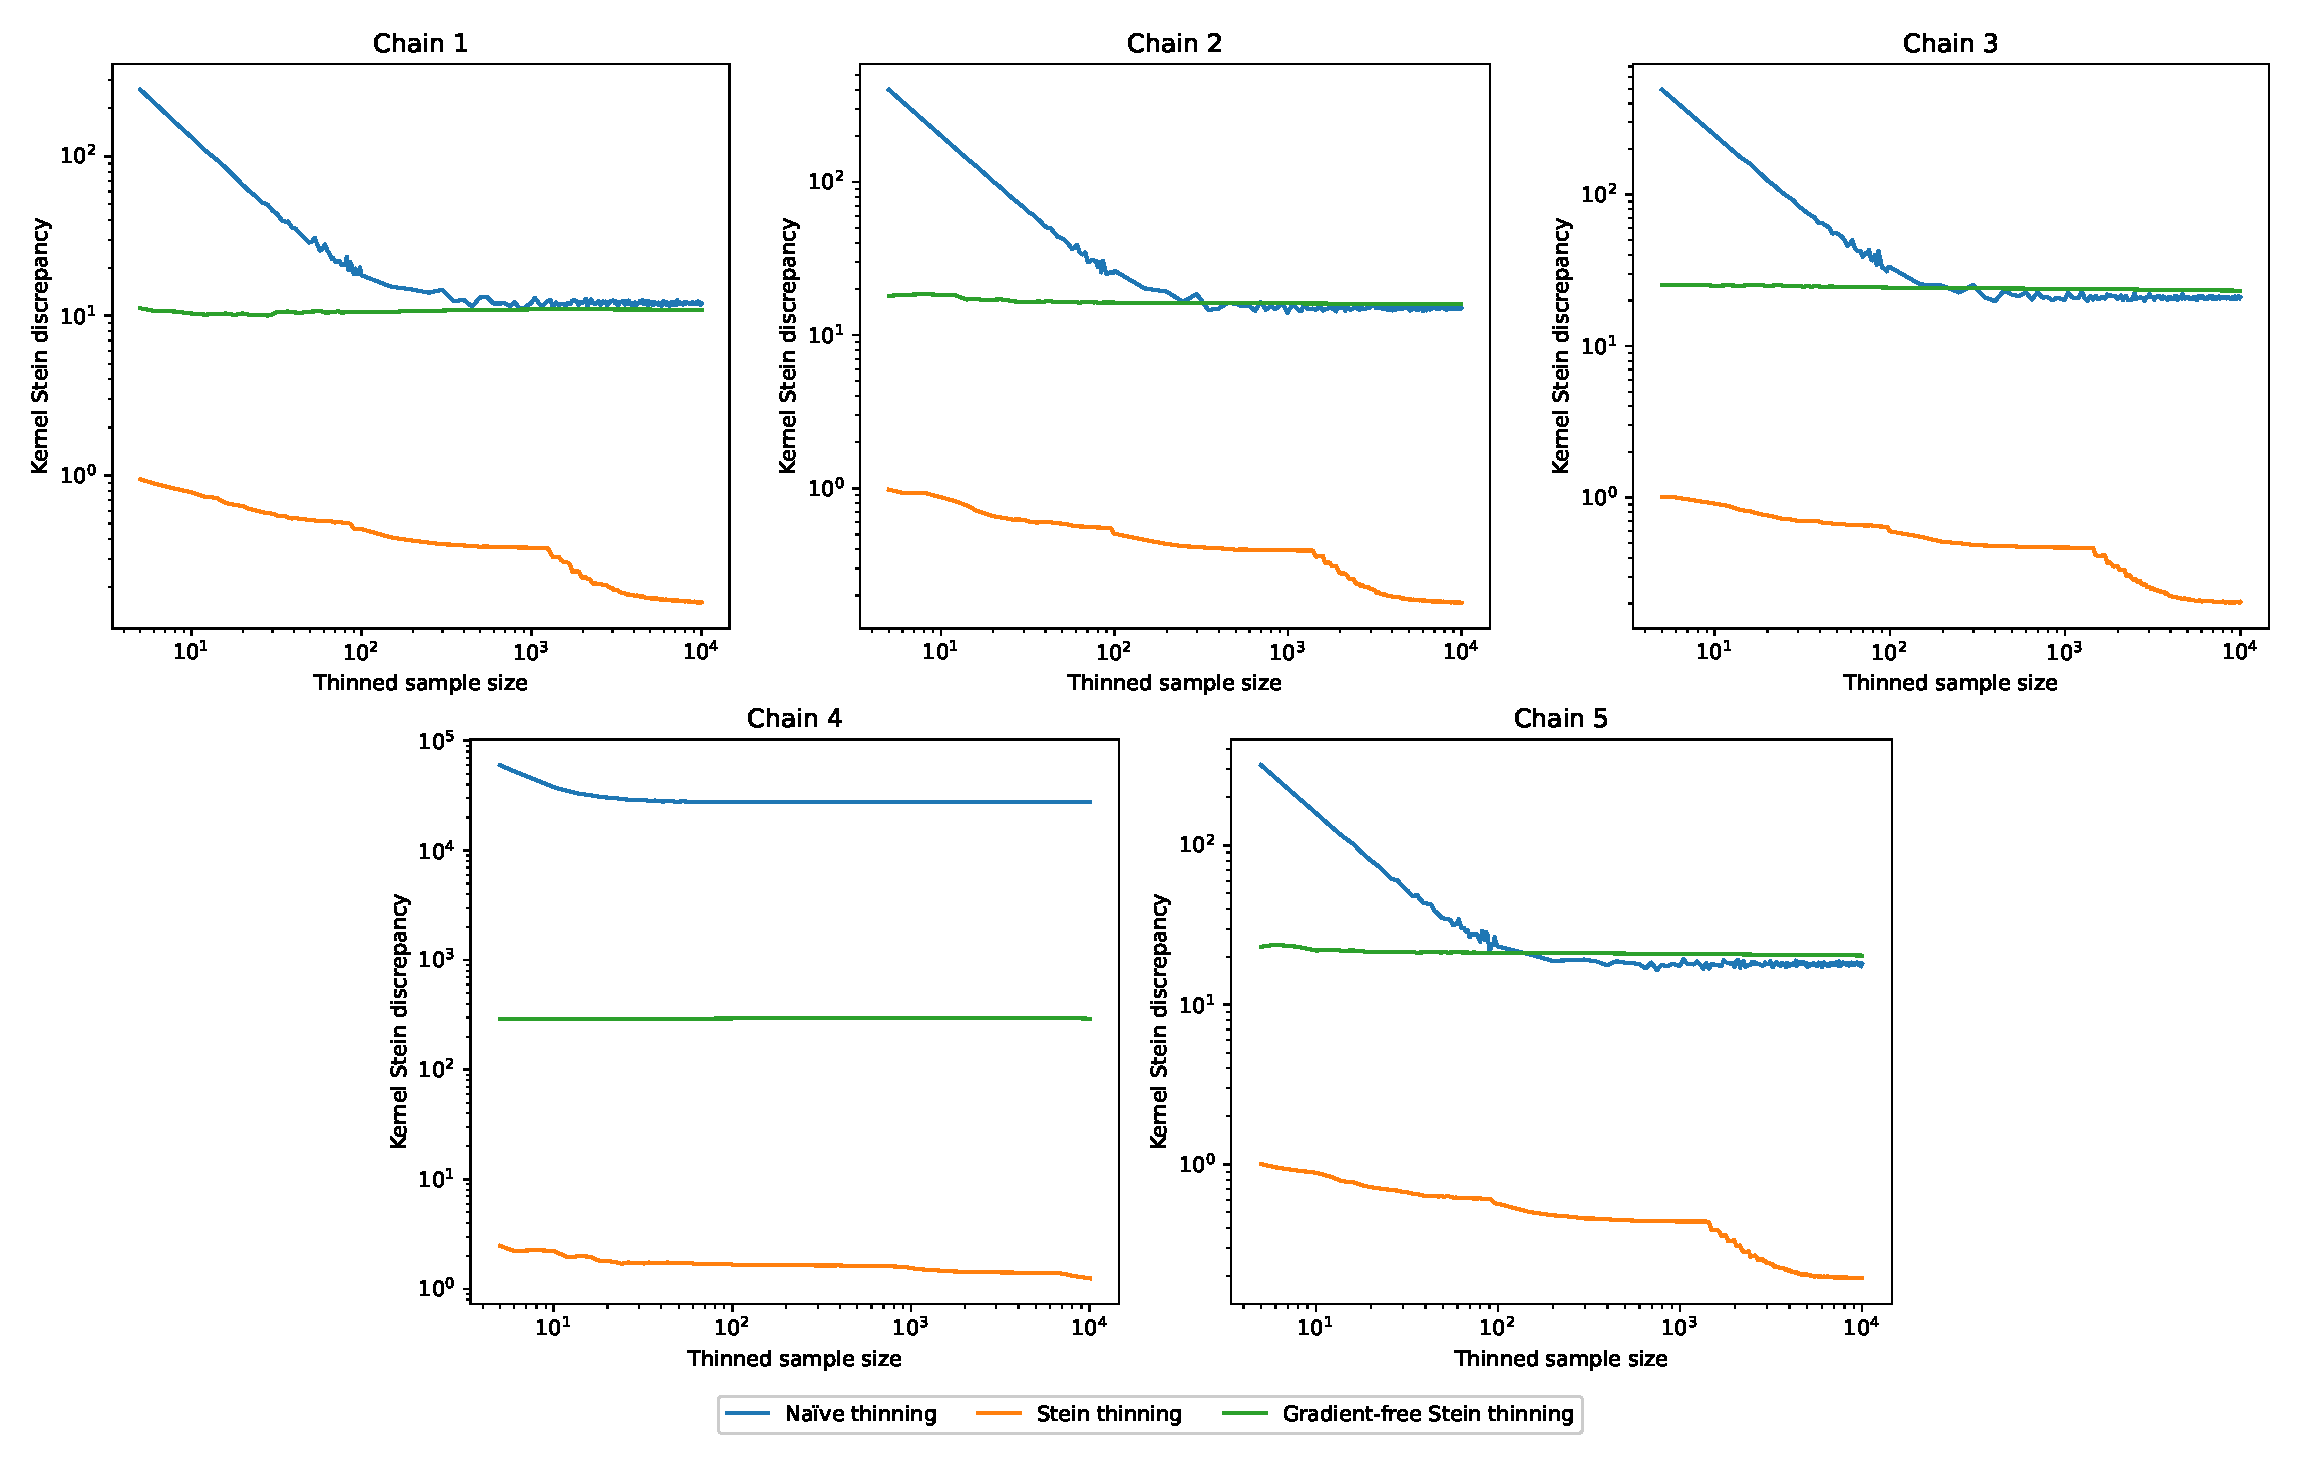
\includegraphics[width=1.0\textwidth]{lotka-volterra-gf-thinning-ksd.eps}
}
\caption{Kernel Stein discrepancy comparison between gradient-free and standard Stein thinning for the Lotka-Volterra inverse problem.
\label{fig:lotka-volterra:gf-thinning:ksd}}
\end{figure}

We conclude again that a good choice of an auxiliary distribution is key for applying the gradient-free algorithm successfully. A multivariate Gaussian distribution using the sample mean and covariance offer a good starting point for the Lotka-Volterra problem, whereas the approach based on KDE imposes a substantial computational cost and the Laplace approximation fails to produce a thinned sample.

\chapter{Conclusions and Further Work}
\label{ch:conclusions}

This dissertation makes two contributions. We implement the gradient-free Stein thinning algorithm in the Python library \texttt{stein-thinning} and evaluate the performance of the proposed algorithm for i.i.d.\ samples from a Gaussian mixture and MCMC samples from the Lotka-Volterra inverse problem. In addition, we optimise the performance of the existing Stein thinning algorithm to reduce its computational cost from $O(nm^2)$ to $O(nm)$, where $n$ is the input sample size and $m$ is the desired thinned sample size.

We conclude that the gradient-free approach is feasible and performs similarly to the Stein thinning algorithm of \cite{riabizOptimalThinningMCMC2022} for small thinned sample sizes, however its performance depends crucially on the choice of the auxiliary distribution. Even in the highly favourable setting of i.i.d.\ samples from a Gaussian mixture for instance, choosing the auxiliary distribution based on the Laplace approximation fails to produce a thinned sample. While the simple multivariate Gaussian distribution using the sample mean and covariance offers a good starting point, bespoke treatment might be required for more complex problems. In deciding whether to use the new algorithm as opposed to the gradient-based approach, the effort involved in selecting a good auxiliary distribution must be weighed against the computational cost of obtaining gradients.

Many interesting avenues for further research remain open:

\textit{Evaluate the choices of KDE kernels other than Gaussian for constructing the auxiliary distribution.} Kernels with bounded support (uniform, saw-tooth, Epanechnikov) are expected to be of limited use, since they do not provide gradient estimates outside of their support, however fat-tailed kernels (e.g. exponential or Student's $t$) are an interesting option to consider.

\textit{Parallelise the computation of KDE.} As noted in \Cref{sec:lotka-volterra}, the computational cost of the KDE approach rises as $O(n^2)$, where $n$ is the size of the sample. Evaluations of the density, however, can be performed in parallel, extending the range of sample sizes that can be handled within a given time budget.

\textit{Perform thinning in a lower-dimensional space.} Samples from the MCMC runs for the Lotka-Volterra problem (see \Cref{fig:lotka-volterra:chain1-sample}, for example) indicate correlation between the parameters. Methods of dimensionality reduction, such as principal component analysis (PCA), could be used to identify a lower-dimensional representation of the samples, and thinning could be done in the transformed space.

\textit{Investigate the behaviour of Stein thinning for large thinned sample sizes}. An interesting feature of \Cref{fig:lotka-volterra:stein-thinning:energy-distance} that warrants further investigation is that the energy distance for the gradient-based algorithm remains approximately constant up to sample sizes around 1000, and then starts reducing further.

\textit{Compare the performance of the approaches in terms of estimating the true parameters of the Lotka-Volterra model.} While the energy distance offers a richer metric of dissimilarity between distributions, parameter inference is often the goal in practice, so a simple comparison between first moment estimates could be useful.

\textit{Run an experiment with randomised starting points}. Building on the preceding idea, one could try initialising a large number of chains with starting values drawn from some distribution, perform sampling and thinning, and compare the mean-squared errors of the resulting parameter estimates.

\textit{Repeat the experiments in \Cref{sec:lotka-volterra} with more advanced MCMC algorithms}. For example, the MALA sampler considered in \cite{riabizOptimalThinningMCMC2022} or the HMC sampler implemented in the \texttt{PyStan} library could be used.

\textit{Check how running a gradient-free MCMC sampling algorithm (such the random-walk Metropolis-Hastings) followed by Stein thinning of the sample compares to running a gradient-based sampling algorithm (e.g. HMC).} Given the sequential nature of MCMC, the costs of calculating the gradients add up in the later case, but can be parallelised in the former. It would be interesting to see which approach produces higher-quality samples under a fixed time budget.

\textit{Provide theoretical justification for gradient-free Stein thinning}. This involves proving the equivalent of Theorem 4 in \cite{chenSteinPointMarkov2019} to show that the preconditioner matrix can be used in the gradient-free algorithm, and demonstrating the bias-correction result of Theorem 3 in \cite{riabizOptimalThinningMCMC2022} for gradient-free Stein thinning.

\textit{Explore other gradient-free alternatives.} A promising approach by \cite{huangEnhancingSampleQuality2023} involves selecting importance weights by viewing the points of the sample as charged particles and minimising the total potential energy of their configuration. The resulting convex quadratic programming problem can be solved efficiently.


\bibliographystyle{plainnat_modified}
\bibliography{biblio}

\appendix

\chapter{Derivations}
\label{appendix:derivations}

\section{Stein kernel based on inverse multiquadric kernel}
\label{appendix:derivations:imq-stein}

When $k(x,y)$ is the inverse multiquadric kernel~(\ref{eq:imq}) with $x, y \in \mathbb{R}^d$, the corresponding Stein kernel $k_P(x, y)$ is obtained from~(\ref{eq:deriv:stein-kernel}). We start by evaluating the terms in (\ref{eq:deriv:stein-kernel}). First, for $r \in \{1, \dots, d\}$,
\begin{equation}
\begin{aligned}
\frac{\partial^2}{\partial x_r\,\partial y_r} k(x,y) 
= &-4 \beta(\beta-1) \left(c^2 + \sum_{i=1}^d\sum_{j=1}^d (x_i-y_i) \Gamma^{-1}_{ij}(x_j-y_j)\right)^{\beta-2} \left(\sum_{j=1}^d \Gamma^{-1}_{rj}(x_j - y_j)\right)^2 \\
&- 2\beta \left(c^2 + \sum_{i=1}^d\sum_{j=1}^d (x_i-y_i) \Gamma^{-1}_{ij}(x_j-y_j)\right)^{\beta-1} \Gamma^{-1}_{rr}
\end{aligned}
\end{equation}
which gives us
\begin{equation}
\begin{aligned}
(\nabla_x \cdot \nabla_y) k(x,y) 
&= -4 \beta(\beta-1) \left(c^2 + \| \Gamma^{-1/2}(x-y)\|^2\right)^{\beta-2} \| \Gamma^{-1}(x - y)\|^2 \\
&- 2\beta \left(c^2 + \|\Gamma^{-1/2}(x-y)\|^2\right)^{\beta-1} \trace(\Gamma^{-1})
\label{eq:appx:deriv:nablax_nablay}
\end{aligned}
\end{equation}
Now,
\begin{equation}
\begin{aligned}
\frac{\partial}{\partial x_r} k(x,y) 
%&= \beta \left(c^2 + \sum_{i=1}^d\sum_{j=1}^d (x_i-y_i) \Gamma^{-1}_{ij}(x_j-y_j)\right)^{\beta-1} \\
%&\times \left( \sum_{j=1}^d \Gamma^{-1}_{lj}(x_j - y_j) + \sum_{i=1}^d (x_i - x_j) \Gamma^{-1}_{il} \right) \\
&= \beta \left(c^2 + \sum_{i=1}^d\sum_{j=1}^d (x_i-y_i) \Gamma^{-1}_{ij}(x_j-y_j)\right)^{\beta-1}
\sum_{j=1}^d (\Gamma^{-1} + \Gamma^{-T})_{rj}(x_j - y_j) \\
&= 2 \beta \left(c^2 + \sum_{i=1}^d\sum_{j=1}^d (x_i-y_i) \Gamma^{-1}_{ij}(x_j-y_j)\right)^{\beta-1}
\sum_{j=1}^d \Gamma^{-1}_{rj}(x_j - y_j), \\
\end{aligned}
\end{equation}
where we used that $\Gamma$ is a symmetric matrix. The gradient is then
\begin{equation}
\nabla_x k(x,y) = 2 \beta \left(c^2 + \| \Gamma^{-1/2} (x-y)\|^2\right)^{\beta-1} \Gamma^{-1} (x - y).
\label{eq:appx:deviv:nablax}
\end{equation}
and similarly
\begin{equation}
\nabla_y k(x,y) = -2 \beta \left(c^2 + \| \Gamma^{-1/2} (x-y)\|^2\right)^{\beta-1} \Gamma^{-1} (x - y).
\label{eq:appx:deviv:nablay}
\end{equation}

Substituting (\ref{eq:appx:deviv:nablax}), (\ref{eq:appx:deviv:nablay}) and (\ref{eq:appx:deriv:nablax_nablay}) into (\ref{eq:deriv:stein-kernel}), we obtain
\begin{equation}
\begin{aligned}
k_P(x, y)
= &-4 \beta(\beta-1) \left(c^2 + \| \Gamma^{-1/2}(x-y)\|^2\right)^{\beta-2} \| \Gamma^{-1}(x - y)\|^2 \\
&- 2\beta \left(c^2 + \|\Gamma^{-1/2}(x-y)\|^2\right)^{\beta-1} \trace(\Gamma^{-1}) \\
&+ 2 \beta \left(c^2 + \| \Gamma^{-1/2} (x-y)\|^2\right)^{\beta-1} \langle \Gamma^{-1} (x - y), \nabla_y \log p(y)\rangle \\
&- 2 \beta \left(c^2 + \| \Gamma^{-1/2} (x-y)\|^2\right)^{\beta-1} \langle \Gamma^{-1} (x - y), \nabla_x \log p(x)\rangle \\
&+ \left(c^2 + \| \Gamma^{-1/2} (x-y)\|^2\right)^\beta \langle \nabla_x \log p(x), \nabla_y \log p(y) \rangle \\
= &-4 \beta(\beta-1) D^{\beta-2} \| \Gamma^{-1}(x - y)\|^2  \\
&- 2 \beta D^{\beta-1} (\trace(\Gamma^{-1}) + \langle \Gamma^{-1} (x - y), \nabla_x \log p(x) - \nabla_y \log p(y)\rangle) \\
&+ D^\beta \langle \nabla_x \log p(x), \nabla_y \log p(y) \rangle, \\
\end{aligned}
\label{eq:k_P:IMQ}
\end{equation}
where in the last equation we have denoted $D = c^2 + \| \Gamma^{-1/2}(x-y)\|^2$.

\section{Gradient of the Gaussian mixture distribution}
\label{appendix:derivations:gaussian-mixture-gradient}

For multivariate normal distributions with density functions
$$f_i(x) = \frac{1}{(2\pi)^{d/2} |\Sigma_i|^{1/2}}\exp\left(-\frac{1}{2}(x - \mu_i)^T \Sigma_i^{-1}(x - \mu_i)\right),$$
where $x \in \mathbb{R}^d$, the mixture density with $k$ components is given by
$$f(x) = \sum_{i=1}^k w_i f_i(x),$$
thus the gradient of its log-density is obtained as
$$\nabla_{x} \log f(x) = \frac{\sum_{i=1}^k w_i \nabla_{x} f_i(x)}{\sum_{i=1}^k w_i f_i(x)} = -\frac{\sum_{i=1}^k w_i f_i(x) \Sigma_i^{-1}(x - \mu_i)}{\sum_{i=1}^k w_i f_i(x)}.$$

\section{Forward sensitivity equations for the Lotka-Volterra model}
\label{appendix:derivations:forward-sensitivity}

Given a system of ODEs of the form:
$$\frac{\diff u_r}{\diff t} = F_r(t, u_1, \dots, u_q; \theta_1, \dots, \theta_d),\qquad r=1,\dots,q,$$
where $q$ is the dimension of the state space (i.e.\ the number of observed variables) and $d$ is the dimension of the parameter space,
the sensitivities can be found by solving forward sensitivity equations:
$$\frac{\diff}{\diff t}\left(\frac{\partial u_r}{\partial \theta_s}\right)
= \frac{\partial}{\partial \theta_s}\frac{\diff u_r}{\diff t} 
%= \frac{\diff F_r}{\diff \theta_s} 
= \frac{\partial F_r}{\partial \theta_s} + \sum_{l=1}^q \frac{\partial F_r}{\partial u_l} \frac{\partial u_l}{\partial \theta_s}.$$

For the Lotka-Volterra model~(\ref{eq:lotka-volterra}), this yields eight additional equations:
\begin{equation*}
\begin{aligned}
\frac{\diff}{\diff t}\left(\frac{\partial u_1}{\partial \theta_1}\right) &= u_1 + (\theta_1 - \theta_2 u_2) \frac{\partial u_1}{\partial \theta_1} - \theta_2 u_1 \frac{\partial u_2}{\partial \theta_1}, \\
\frac{\diff}{\diff t}\left(\frac{\partial u_1}{\partial \theta_2}\right) &= - u_1 u_2 + (\theta_1 - \theta_2 u_2) \frac{\partial u_1}{\partial \theta_2} - \theta_2 u_1 \frac{\partial u_2}{\partial \theta_2}, \\
\frac{\diff}{\diff t}\left(\frac{\partial u_1}{\partial \theta_3}\right) &= (\theta_1 - \theta_2 u_2) \frac{\partial u_1}{\partial \theta_3} - \theta_2 u_1 \frac{\partial u_2}{\partial \theta_3}, \\
\frac{\diff}{\diff t}\left(\frac{\partial u_1}{\partial \theta_4}\right) &= (\theta_1 - \theta_2 u_2) \frac{\partial u_1}{\partial \theta_4} - \theta_2 u_1 \frac{\partial u_2}{\partial \theta_4}, \\
\frac{\diff}{\diff t}\left(\frac{\partial u_2}{\partial \theta_1}\right) &= \theta_4 u_2 \frac{\partial u_1}{\partial \theta_1} + (\theta_4 u_1 - \theta_3) \frac{\partial u_2}{\partial \theta_1}, \\
\frac{\diff}{\diff t}\left(\frac{\partial u_2}{\partial \theta_2}\right) &= \theta_4 u_2 \frac{\partial u_1}{\partial \theta_2} + (\theta_4 u_1 - \theta_3) \frac{\partial u_2}{\partial \theta_2}, \\
\frac{\diff}{\diff t}\left(\frac{\partial u_2}{\partial \theta_3}\right) &= -u_2 + \theta_4 u_2 \frac{\partial u_1}{\partial \theta_3} + (\theta_4 u_1 - \theta_3) \frac{\partial u_2}{\partial \theta_3}, \\
\frac{\diff}{\diff t}\left(\frac{\partial u_2}{\partial \theta_4}\right) &= u_1 u_2 + \theta_4 u_2 \frac{\partial u_1}{\partial \theta_4} + (\theta_4 u_1 - \theta_3) \frac{\partial u_2}{\partial \theta_4}. \\
\end{aligned}
\end{equation*}

\chapter{Additional figures}
\label{appendix:figures}

\Cref{fig:gmm:laplace:first-iterations} shows the values used in the first two optimisation steps of \Cref{alg:gf} for the bivariate Gaussian mixture of \Cref{sec:gaussian-mixture} with the auxiliary distribution based on the Laplace approximation. Specifically, the first iteration selects $i$ that minimises
\begin{equation*}
\frac{k_Q(x_i, x_i)}{2},
\end{equation*}
whereas the second iteration minimises
\begin{equation*}
\frac{k_{P,Q}(x_i, x_i)}{2} + k_{P,Q}(x_{\pi(1)}, x_i),
\end{equation*}
where $\pi(1)$ is the index of the element selected on the first iteration. The same element ends up selected on both iterations.

\begin{figure}[h]
\centering
\makebox[\textwidth][c]{
	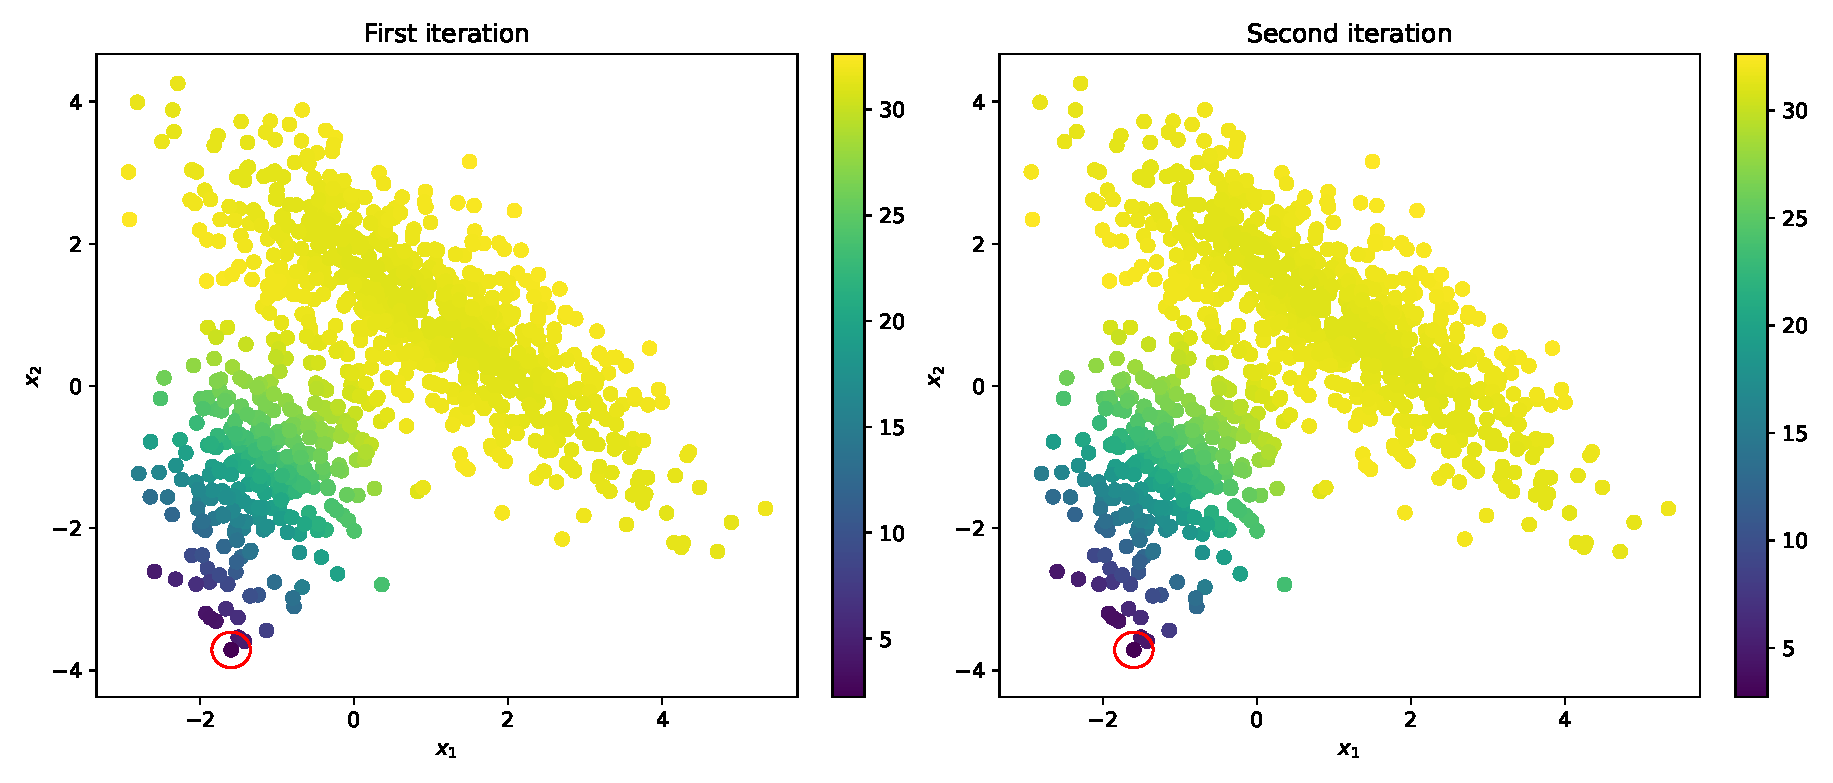
\includegraphics[width=1.0\textwidth]{gaussian-mixture-laplace-first-iterations.eps}
}
\caption{Values used in the first two optimisation steps of the Stein thinning algorithm for the bivariate Gaussian mixture with the auxiliary distribution based on the Laplace approximation. The values are shown in the $\log_{10}$ scale. The element selected by the optimisation in both cases is circled.
\label{fig:gmm:laplace:first-iterations}}
\end{figure}

\begin{figure}[h]
\centering
\makebox[\textwidth][c]{
	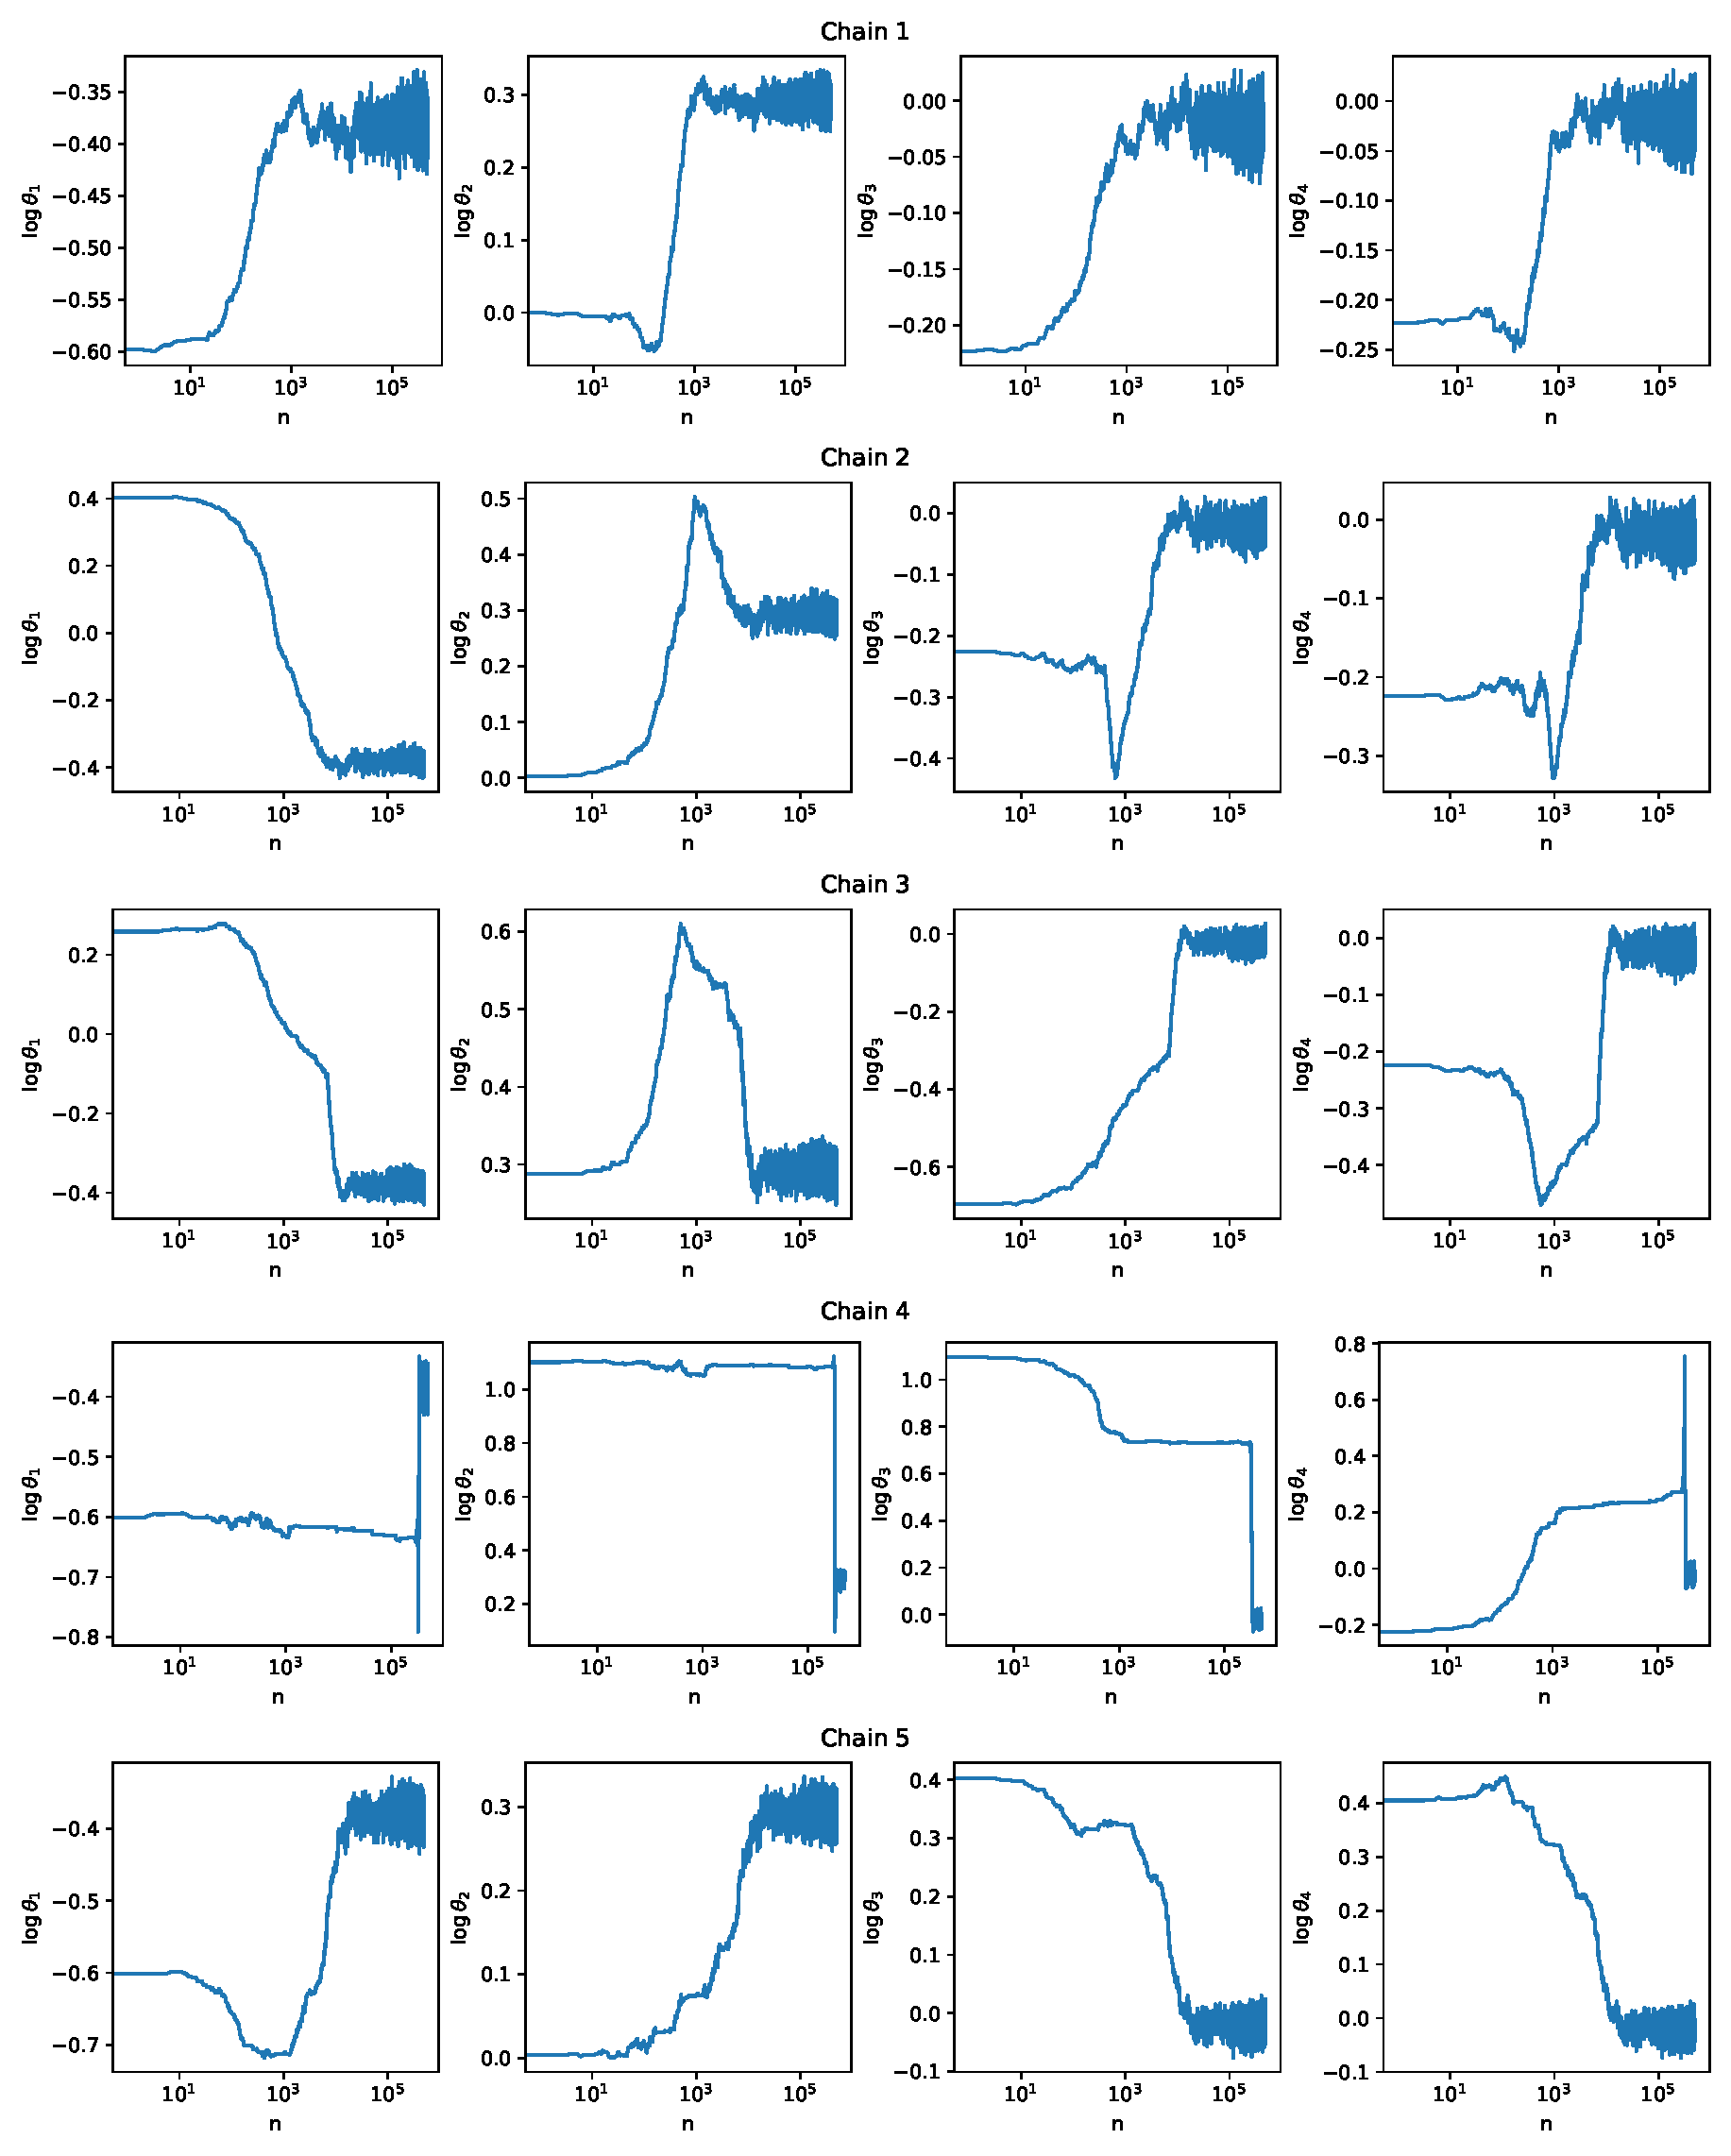
\includegraphics[width=1.0\textwidth]{lotka-volterra-trace-plots.eps}
}
\caption{Trace plots from the random-walk Metropolis-Hastings algorithm for the Lotka-Volterra inverse problem.
\label{fig:lotka-volterra:trace-plots}}
\end{figure}

\begin{figure}[h]
\centering
\makebox[\textwidth][c]{
	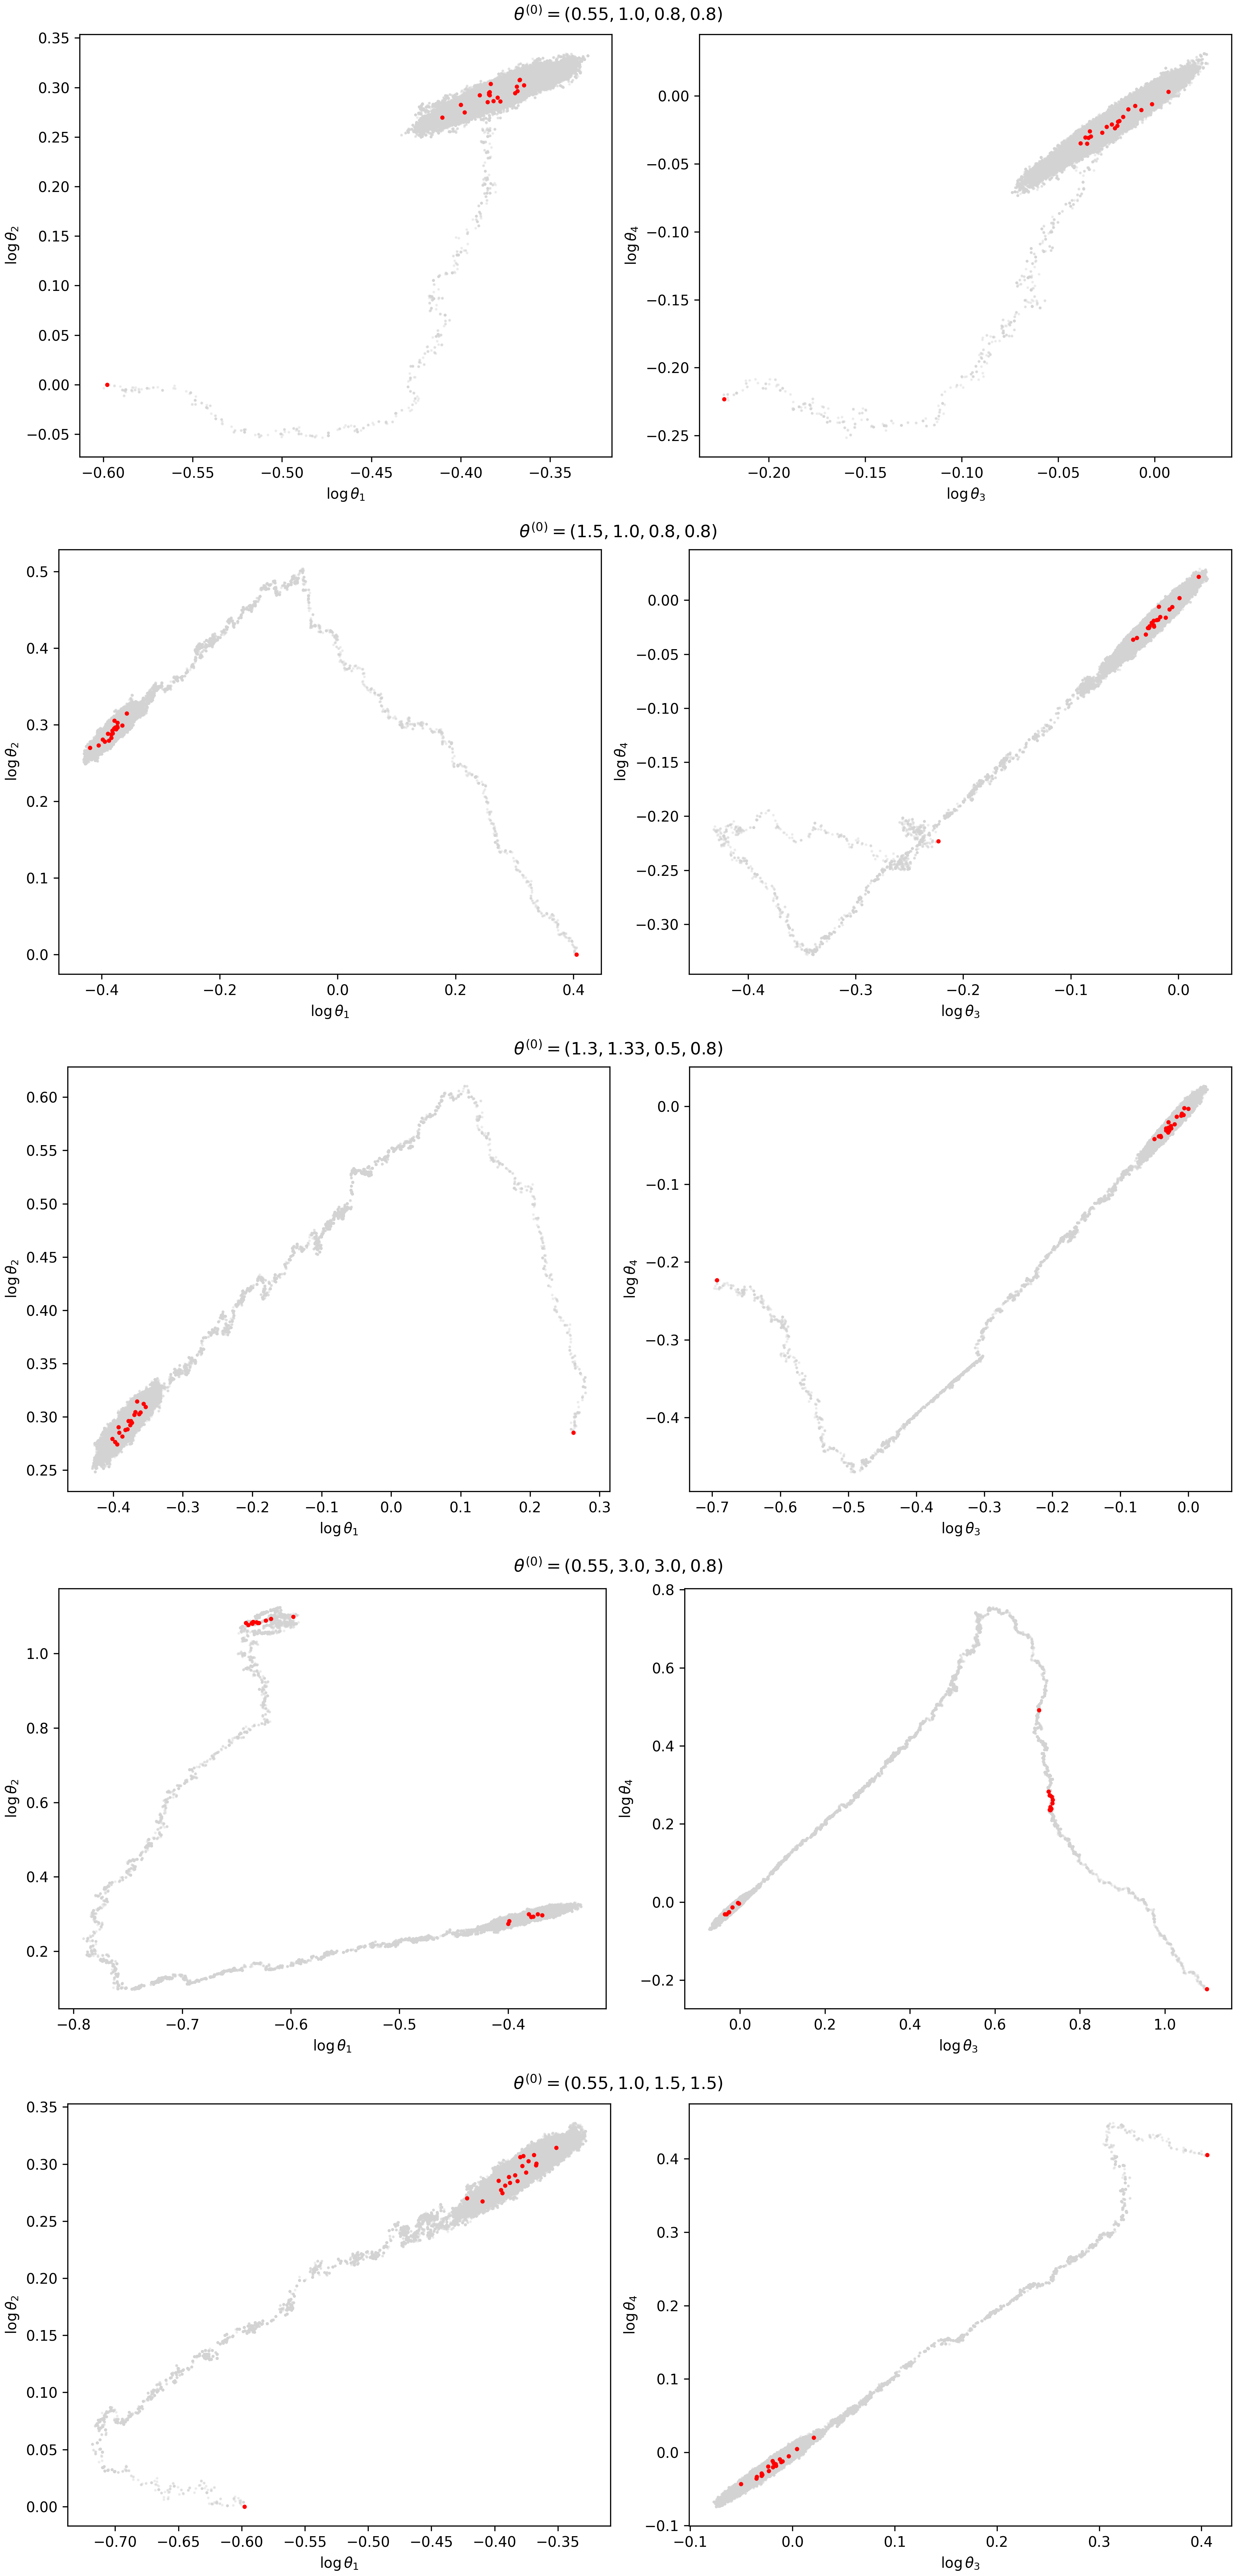
\includegraphics[height=.9\textheight]{lotka-volterra-naive-thinning.png}
}
\caption{Results of na\"ive thinning of the sample from the Lotka-Volterra model.
\label{fig:lotka-volterra:naive:results}}
\end{figure}

\begin{figure}[h]
\centering
\makebox[\textwidth][c]{
	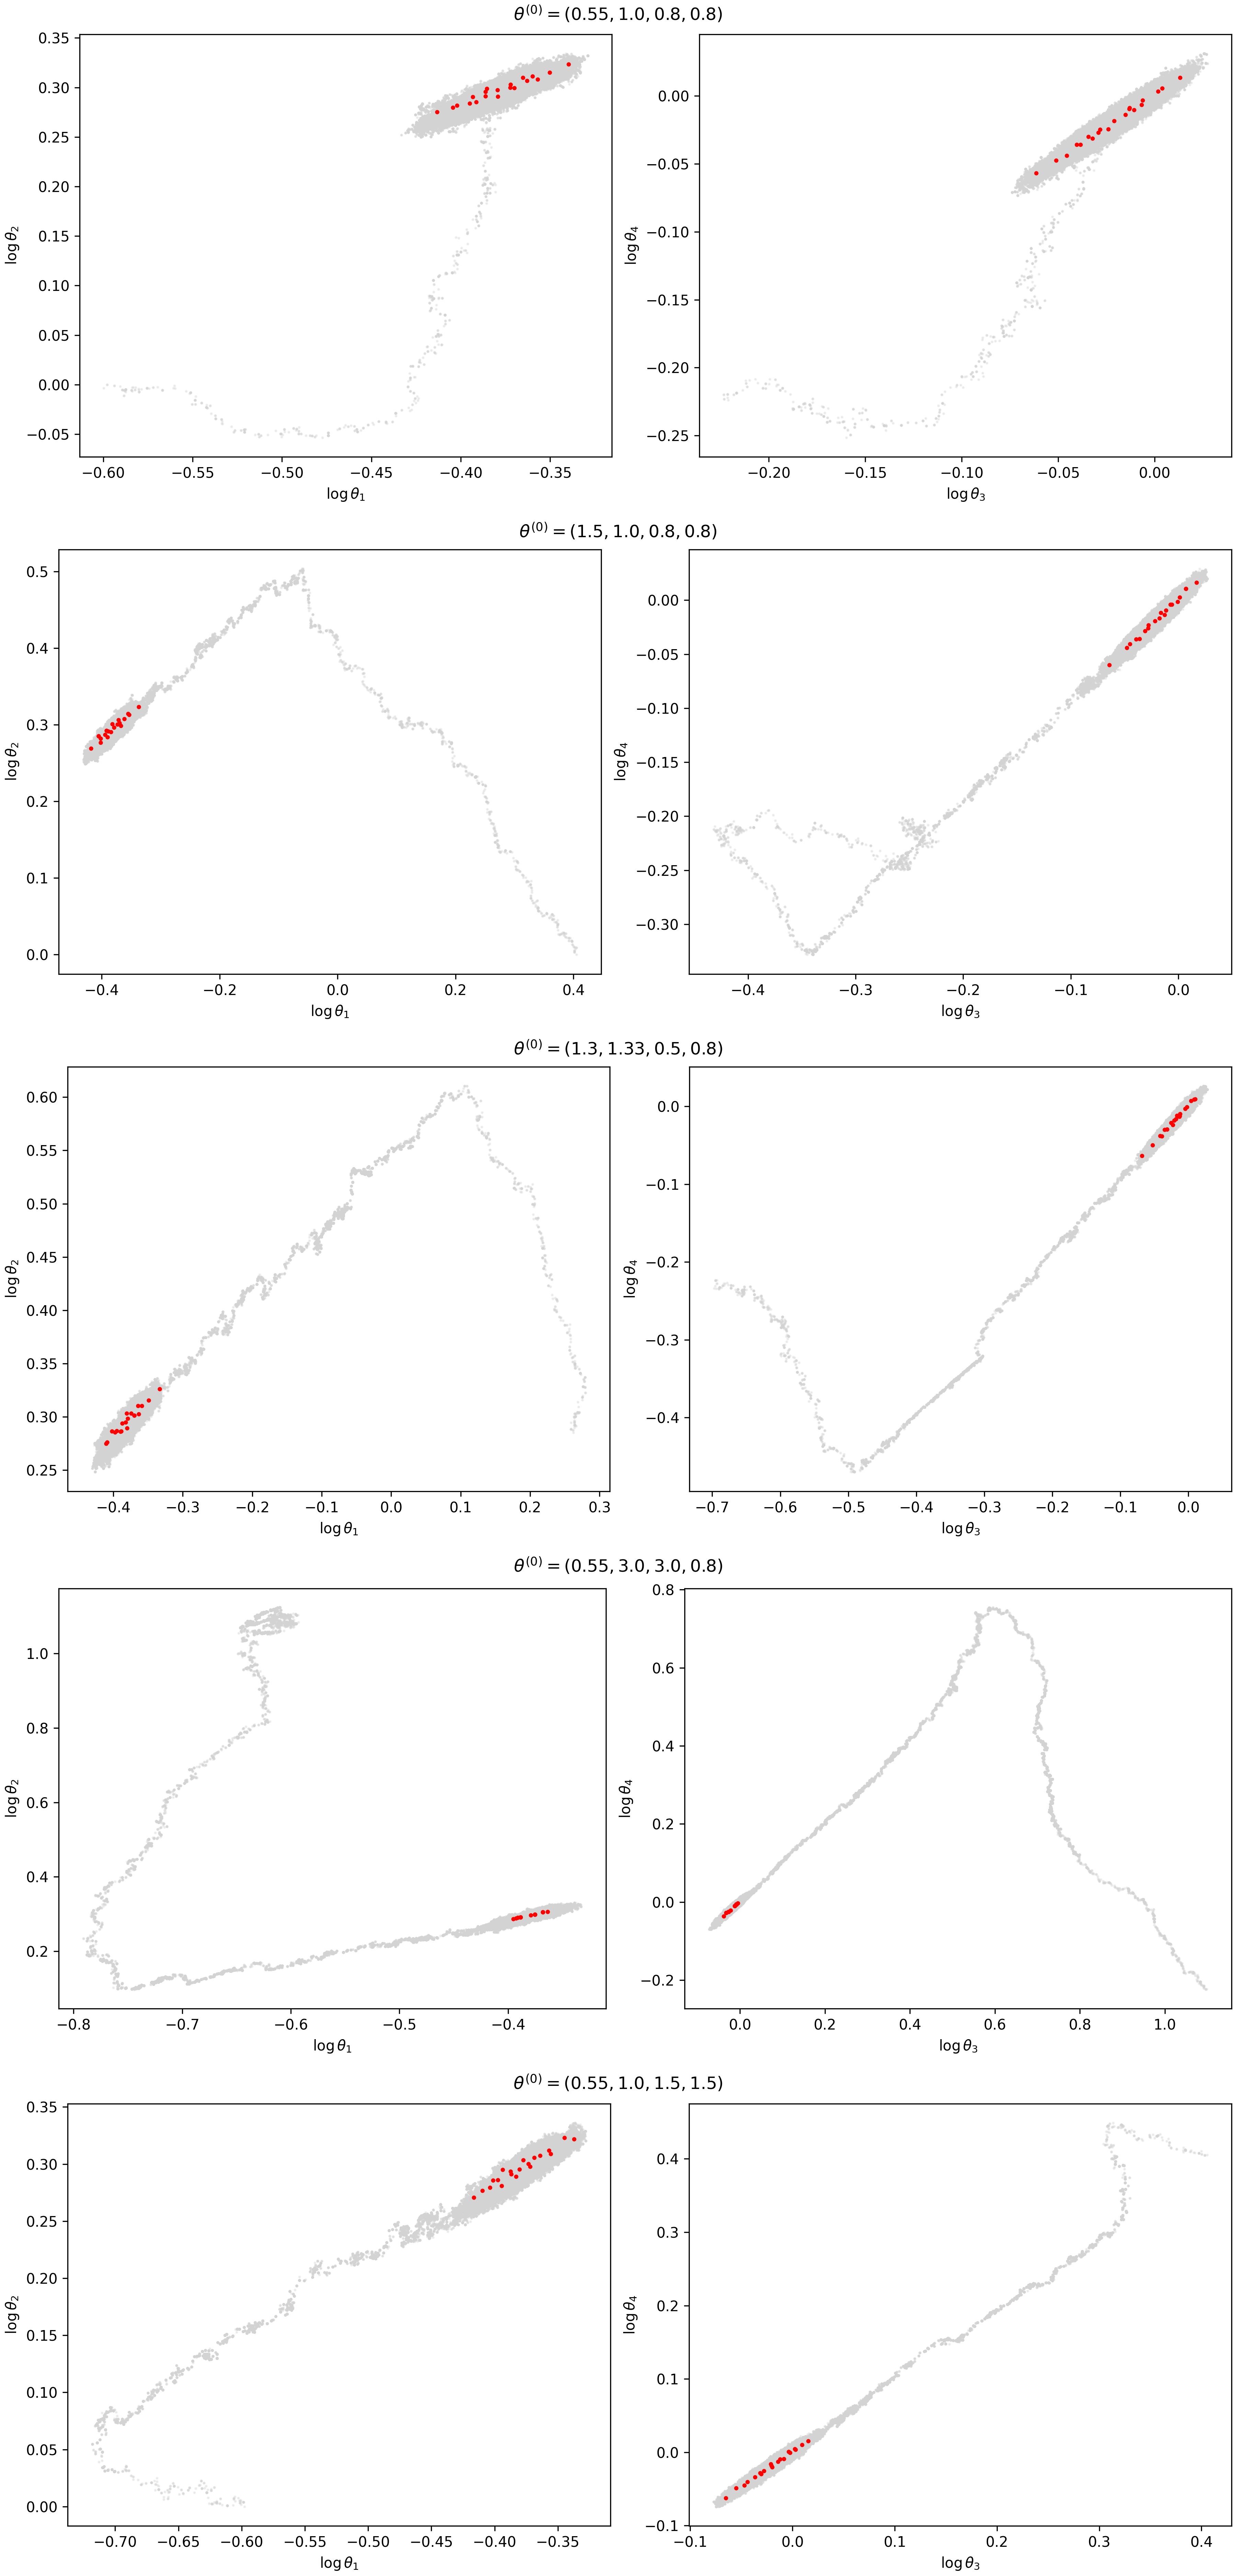
\includegraphics[height=.9\textheight]{lotka-volterra-stein-thinning.png}
}
\caption{The first 20 points selected by the Stein thinning algorithm for each MCMC chain in the Lotka-Volterra inverse problem.
\label{fig:lotka-volterra:stein:results}}
\end{figure}

\end{document}
